\documentclass[aspectratio=169]{beamer}
% \usepackage[utf8]{inputenc}
\usetheme{metropolis}
\usecolortheme{orchid}
\usepackage{amsmath}
\usepackage{amssymb}
\usepackage{amsthm}
\usepackage{multirow}
\usepackage[ruled]{algorithm2e}
\usepackage{mathtools}
\usepackage{caption}
% \usepackage{epstopdf}
\usepackage{hyperref}
\usepackage{subcaption}
\usepackage{siunitx}
\usepackage{textcomp}
\usepackage{tcolorbox}
\usepackage{tikz}
\usetikzlibrary{tikzmark,positioning,arrows.meta,shapes.misc,calc}

\setbeamerfont{footnote}{size=\tiny}

% Information boxes
\newcommand*{\info}[4][16.3]{%
  \node [ annotation, #3, scale=0.65, text width = #1em,
          inner sep = 2mm ] at (#2) {%
  \list{$\bullet$}{\topsep=0pt\itemsep=0pt\parsep=0pt
    \parskip=0pt\labelwidth=8pt\leftmargin=8pt
    \itemindent=0pt\labelsep=2pt}%
    #4
  \endlist
  };
}

%% Definitions for root locus plots
\newcommand*{\rootlocusexample}[4]{% xmin,xmax,ymin,ymax,
		\foreach \x in {#1,...,#2}{
			\ifthenelse{\x=0}{}
		  {% false case
   			\draw (\x cm,1pt) -- (\x cm,-1pt) node[anchor=north] {$\x$};
		  }
		}
		\foreach \y in {#3,...,#4}{
			\ifthenelse{\y=0}{}
		  {% false case
   			\draw (-1pt,\y cm) -- (1pt,\y cm) node[anchor=east] {$\y$};
		  }
   	}
		\draw [-latex] (#1,0) -- (#2,0) node [above]  {$\sigma$};
		\draw [-latex] (0,#3) -- (0,#4) node [right] {$j\omega$};
}

\def\centerarc[#1](#2)(#3:#4:#5)% Syntax: [draw options] (center) (initial angle:final angle:radius)
    { \draw[#1] ($(#2)+({#5*cos(#3)},{#5*sin(#3)})$) arc (#3:#4:#5); }

\tikzset{%
  >={Latex[width=2mm,length=2mm]},
  % Specifications for style of nodes:
            base/.style = {rectangle, rounded corners, draw=black,
                           minimum width=4cm, minimum height=1cm,
                           text centered, font=\sffamily},
  activityStarts/.style = {base, fill=blue!30},
       startstop/.style = {base, fill=red!30},
    activityRuns/.style = {base, fill=green!30},
         process/.style = {base, minimum width=2.5cm, fill=orange!15,
                           font=\ttfamily},
}

\tikzset{pole/.style={cross out, draw=black, minimum size=2*(#1-\pgflinewidth), inner sep=0pt, outer sep=0pt},
pole/.default={3pt}}
\tikzset{poledes/.style={rectangle, draw=black, minimum size=2*(#1-\pgflinewidth), inner sep=0pt, outer sep=0pt},
poledes/.default={3pt}}
\tikzset{zero/.style={circle, draw=black, fill=white, minimum size=2*(#1-\pgflinewidth), inner sep=0pt, outer sep=0pt},
zero/.default={3pt}}
\tikzset{test/.style={rectangle, draw=black, fill=white, minimum size=2*(#1-\pgflinewidth), inner sep=0pt, outer sep=0pt},
test/.default={3pt}}

%% Definitions for block diagrams
\tikzstyle{block} = [draw, fill=blue!20, rectangle, 
    minimum height=2em, minimum width=3em]
\tikzstyle{sum} = [draw, fill=blue!20, circle, node distance=1cm]
\tikzstyle{input} = [coordinate]
\tikzstyle{output} = [coordinate]
\tikzstyle{pinstyle} = [pin edge={to-,thin,black}]

\renewcommand\textbullet{\ensuremath{\bullet}}
\newcommand\scalemath[2]{\scalebox{#1}{\mbox{\ensuremath{\displaystyle #2}}}}
\newcommand{\norm}[1]{\left\lVert#1\right\rVert}

%%% Bibliography
\usepackage[citestyle=numeric,style=numeric,backend=biber,doi=false,isbn=false,url=false]{biblatex}
\addbibresource{references.bib}

%%% Suppress biblatex annoying warning
\usepackage{silence}
\WarningFilter{biblatex}{Patching footnotes failed}

%%% new theorems %%%%%%%%%%%%%%%%%%%%%%%%%%%%%%%%%%%%%%%%%%%%%%%%%%%%%%%%%%%%%%
\theoremstyle{definition}
\newtheorem{mydef}{Definition}

\theoremstyle{plain}
\newtheorem{mylemma}{Lemma}[section]
\newtheorem{mytheorem}{Theorem}[section]
\newtheorem{myproposition}{Proposition}[section]
\newtheorem{myproblem}{Problem}[section]
\newtheorem{mydefinition}{Definition}[section]
\newtheorem{myassumption}{Assumption}[section]

\theoremstyle{remark}
\newtheorem{myremark}{Remark}[section]

\newcounter{saveenumi}
\newcommand{\seti}{\setcounter{saveenumi}{\value{enumi}}}
\newcommand{\conti}{\setcounter{enumi}{\value{saveenumi}}}

\resetcounteronoverlays{saveenumi}

\title{Controles}
\subtitle{\small Clase 8: Respuesta en Frecuencia - Compensadores en Adelanto}
\author{Gerardo Becerra, Ph.D.}
\institute{Pontificia Universidad Javeriana\\ Departamento de Electrónica}
\date{Abril 16, 2020}

\begin{document}

\frame{\titlepage}	

\begin{frame}[<+->]\frametitle{Introducción}
\textbf{Respuesta en frecuencia}
\begin{itemize}
	\item Respuesta estacionaria de un sistema ante una entrada sinusoidal.
	\item Útil para analizar y diseñar sistemas de control.
	\item Generalmente la función de transferencia de sistemas complicados puede obtenerse experimentalmente usando pruebas de respuesta en frecuencia.
	\item Desarrollados en los años 1930s -1940s por Nyquist, Bode, Nichols, entre otros.
	\item No hay una relación directa entre la respuesta en frecuencia y la respuesta en tiempo, excepto para sistemas ideales de segundo orden.
	\item Existen criterios usados durante el diseño de la respuesta en frecuencia para obtener respuestas transitorias en el tiempo aceptables.
\end{itemize}
\end{frame}

\section{Respuesta en Frecuencia}
\begin{frame}[<+->]\frametitle{Respuesta en Frecuencia}
	\begin{figure}
		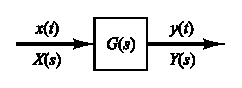
\includegraphics[width=5cm]{images/SLIT.eps}
		\hspace*{10mm}
		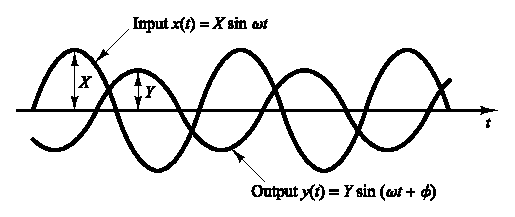
\includegraphics[width=6cm]{images/inputOutputSignals.eps}
	\end{figure}
	\pause
	\begin{itemize}
		\item $\left| G(j\omega) \right| = \left| \frac{Y(j\omega)}{X(j\omega)} \right|$: relación de amplitud de la senoidal de salida respecto a la de entrada.
		\item $\angle G(j\omega) = \angle \left(\frac{Y(j\omega)}{X(j\omega)} \right)$: corrimiento de fase de la senoidal de salida respecto a la de entrada.
		\item $G(j\omega)$: función de transferencia sinusoidal. Se puede obtener reemplazando $s = j\omega$ en la función de transferencia.
	\end{itemize}
\end{frame}

\begin{frame}[<+->]\frametitle{Diagramas de Bode}
	\begin{itemize}
		\item Gráficos logarítmicos que representan de manera simplificada la respuesta en frecuencia de un sistema.
		\item Dos gráficos: logaritmo de la magnitud y fase de la función de transferencia senoidal respecto a la frecuencia en escala logarítmica.
		\item Representación estandar de magnitud de $G(j\omega)$ en decibeles (dB): $20 \log_{10}|G(j\omega)|$.
		\item Ventajas:
		\begin{itemize}
			\item La multiplicación de magnitudes se convierte en suma.
			\begin{equation*}
				20 \log (|G_1(j\omega)G_2(j\omega)|) = 20 \log (|G_1(j\omega)|) + 20 \log (|G_2(j\omega)|)
			\end{equation*}
			\item Existe un método para obtener un bosquejo aproximado del diagrama: suma de respuestas individuales.
			\item La función de transferencia puede obtenerse si existen datos experimentales en la forma del diagrama de Bode.
		\end{itemize}
	\end{itemize}
\end{frame}

\begin{frame}[<+->]\frametitle{Factores Básicos en una Función de Transferencia}
	\begin{equation*}
		G(j\omega) = \frac{K(1+j\omega T_1)}{j\omega(1 + j\omega T_2)(1 + 2\zeta(j\omega/\omega_n)+(j\omega/\omega_n)^2)}
	\end{equation*}
	\pause
	\begin{itemize}
		\item Ganancia $K$
		\item Factores integrales y derivativos $(j\omega)^{\pm 1}$
		\item Factores de primer orden $(1 + j\omega T)^{\pm 1}$
		\item Factores cuadráticos $[1 + 2\zeta(j\omega/\omega_n)+(j\omega/\omega_n)^2]^{\pm 1}$
	\end{itemize}
	\pause
	Es posible utilizar los gráficos logarítmicos de los factores básicos para construir un diagrama de Bode para cualquier función de transferencia $G(j\omega)$ realizando el bosquejo de las curvas de cada factor y luego sumándolas.
\end{frame}

\begin{frame}[<+->]\frametitle{Factores Básicos - Ganancia $K$}
\begin{columns}
	\begin{column}{0.5\textwidth}
	\begin{itemize}
		\item $K > 1$: valor positivo en dB.
		\item $K < 1$: valor negativo en dB.
		\begin{equation*}
			\left| G(j\omega) \right| = 20 \log K
		\end{equation*}
		\begin{equation*}
			\angle G(j\omega) = 0
		\end{equation*}
		\item Variar el valor de $K$ en la función de transferencia $\rightarrow$ sube o baja el gráfico de magnitud un valor constante. No altera el gráfico de magnitud.
	\end{itemize}
	\end{column}
	\begin{column}{0.5\textwidth}
		\begin{figure}
			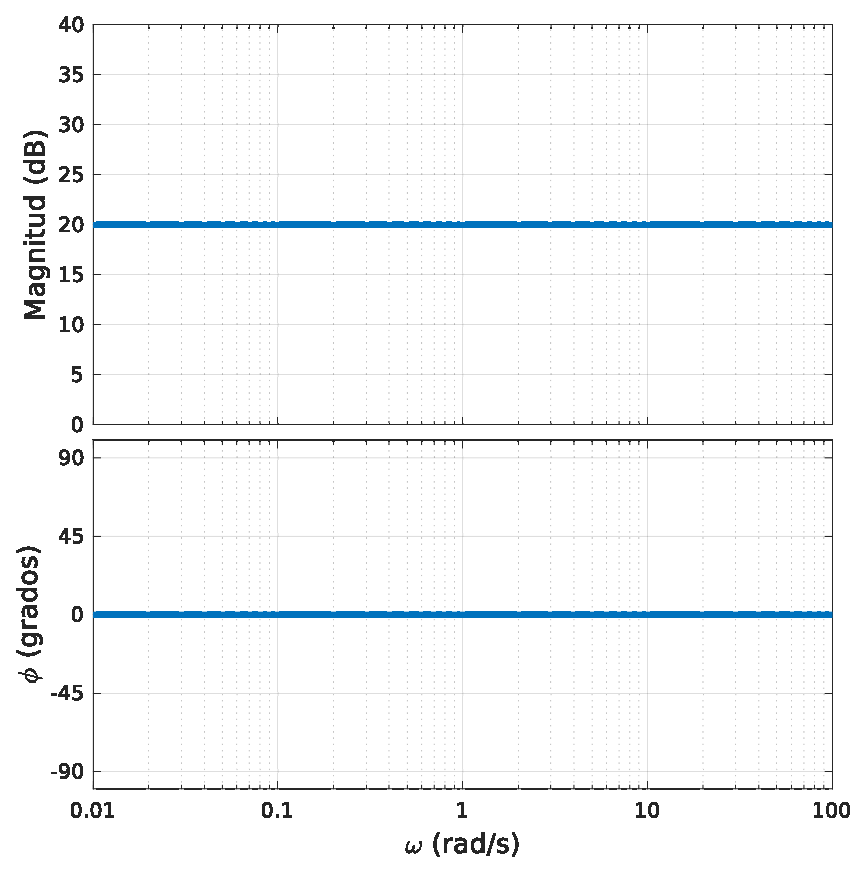
\includegraphics[width=6.5cm]{images/bodeGainK.eps}
		\end{figure}
	\end{column}
\end{columns}
\end{frame}

\begin{frame}[<+->]\frametitle{Factores Básicos - Integral $1/(j\omega)$}
\begin{columns}
	\begin{column}{0.5\textwidth}
	\begin{itemize}
		\item La magnitud logarítmica de $1/j\omega$ es $20\log\left| 1/j\omega \right| = -20 \log \omega$ dB.
		\item La fase de $1/j\omega$ es constante igual a $-\ang{90}$.
		\item Para el caso de $(1/j\omega)^n$:
		\begin{align*}
		  \left| G(j\omega) \right| = 20 \log \left| \frac{1}{(j\omega)^n} \right| &= -20n\log\omega \text{ dB}\\
			\angle G(j\omega) = \angle \left| \frac{1}{(j\omega)^n} \right| &= -n\ang{90}
		\end{align*}
	\end{itemize}
	\end{column}
	\begin{column}{0.5\textwidth}
		\begin{figure}
			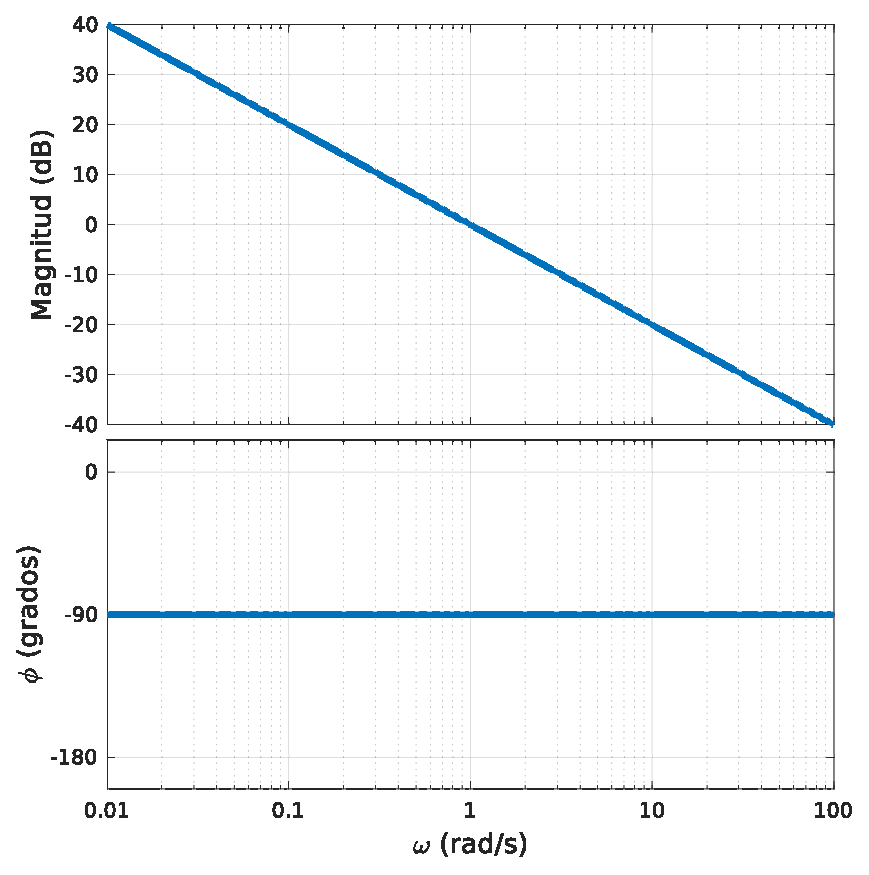
\includegraphics[width=6.5cm]{images/bodeIntegral.eps}
		\end{figure}
	\end{column}
\end{columns}
\end{frame}

\begin{frame}[<+->]\frametitle{Factores Básicos - Derivativo $(j\omega)$}
\begin{columns}
	\begin{column}{0.5\textwidth}
	\begin{itemize}
		\item La magnitud logarítmica de $j\omega$ es $20\log\left| j\omega \right| = 20 \log \omega$ dB.
		\item La fase de $j\omega$ es constante igual a $\ang{90}$.
		\item Para el caso de $(j\omega)^n$:
		\begin{align*}
		  \left| G(j\omega) \right| = 20 \log \left| (j\omega)^n \right| &= 20n\log\omega \text{ dB}\\
			\angle G(j\omega) = \angle \left| (j\omega)^n \right| &= n\ang{90}
		\end{align*}
	\end{itemize}
	\end{column}
	\begin{column}{0.5\textwidth}
		\begin{figure}
			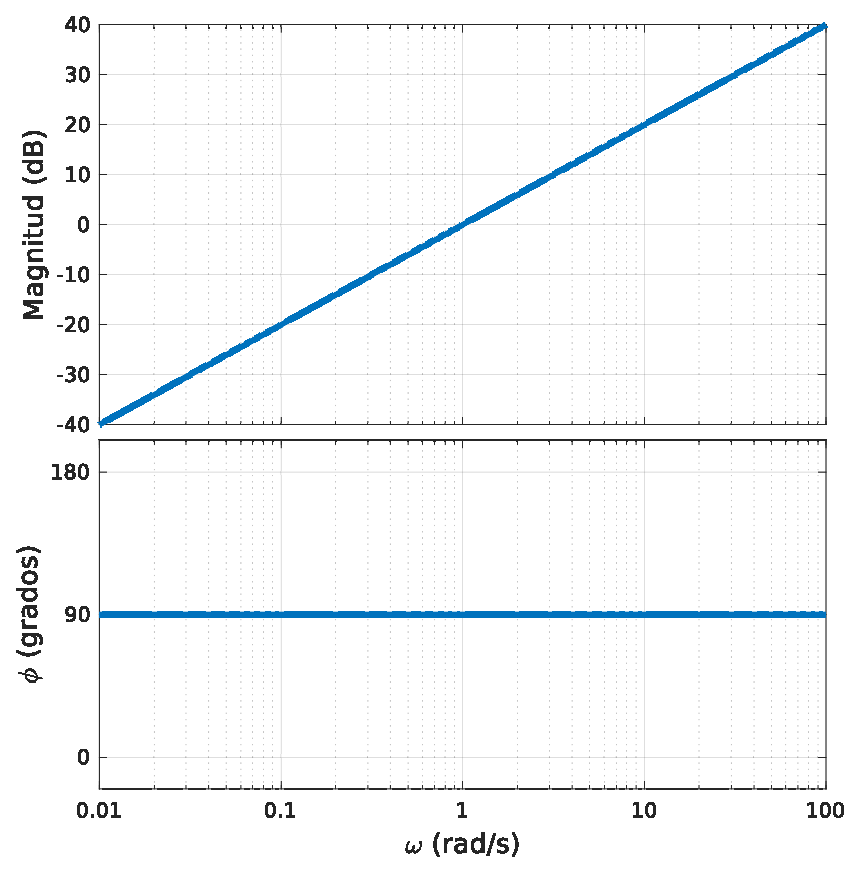
\includegraphics[width=6.5cm]{images/bodeDerivative.eps}
		\end{figure}
	\end{column}
\end{columns}
\end{frame}

\begin{frame}[<+->]\frametitle{Factores Básicos - Primer orden $1/(1+j \omega T)$}
\begin{columns}
	\begin{column}{0.5\textwidth}
	\small
	\begin{itemize}
		\item Magnitud: $\left| G(j\omega) \right| = 20 \log \left| \frac{1}{1+j\omega T} \right|$
		\begin{equation*}
			\left| G(j\omega) \right| = -20 \log \sqrt{1+\omega^2 T^2}
		\end{equation*}
		\item Para bajas frecuencias ($\omega << 1/T$):
		\begin{equation*}
			\left| G(j\omega) \right| = -20 \log 1 = 0 \text{ dB}
		\end{equation*}
		\item Para altas frecuencias ($\omega >> 1/T$):
		\begin{equation*}
			\left| G(j\omega) \right| = -20 \log \omega T \text{ dB}
		\end{equation*}
		\item En la frecuencia de quiebre ($\omega = 1/T$):
		\begin{equation*}
			\left| G(j/T) \right| = - 20\log \sqrt{1 + \frac{T^2}{T^2}} = -3.03 \text{ dB}
		\end{equation*}
	\end{itemize}
	\end{column}
	\begin{column}{0.5\textwidth}
	\centering
	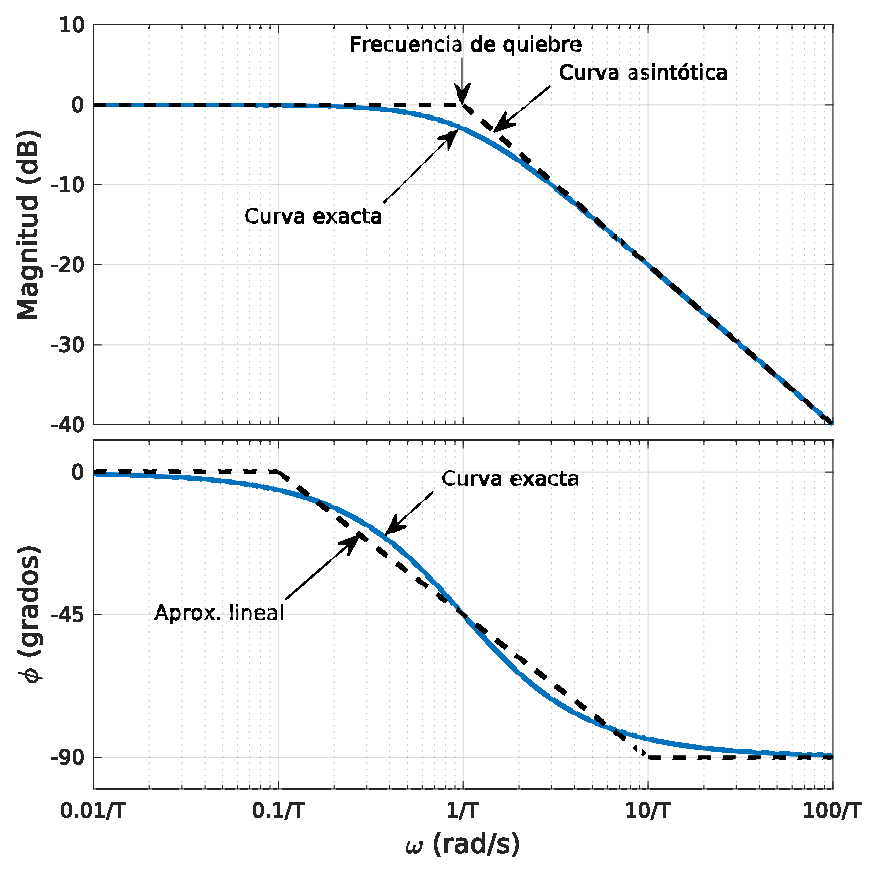
\includegraphics[width=6.5cm]{images/bodeFirstOrderIntegral.eps}
	\end{column}
\end{columns}
\end{frame}

\begin{frame}[<+->]\frametitle{Factores Básicos - Primer orden $1/(1+j \omega T)$}
\vspace*{8mm}
\begin{columns}
	\begin{column}{0.5\textwidth}
	\begin{itemize}
		\item Ángulo de fase: $\phi = -\tan^{-1} \omega T$
		\item Para diferentes frecuencias:
		\begin{align*}
			\omega = 0 \hspace*{3mm} &\Rightarrow \hspace*{3mm} \phi = - \tan^{-1} 0 = \ang{0}\\
			\omega = \frac{1}{T} \hspace*{3mm} &\Rightarrow \hspace*{3mm} \phi = -\tan^{-1}\frac{T}{T} = -\ang{45}\\
			\omega = \infty \hspace*{3mm} &\Rightarrow \hspace*{3mm} \phi = - \tan^{-1} \infty = -\ang{90}
		\end{align*}
	\end{itemize}
	\end{column}
	\begin{column}{0.5\textwidth}
	\centering
	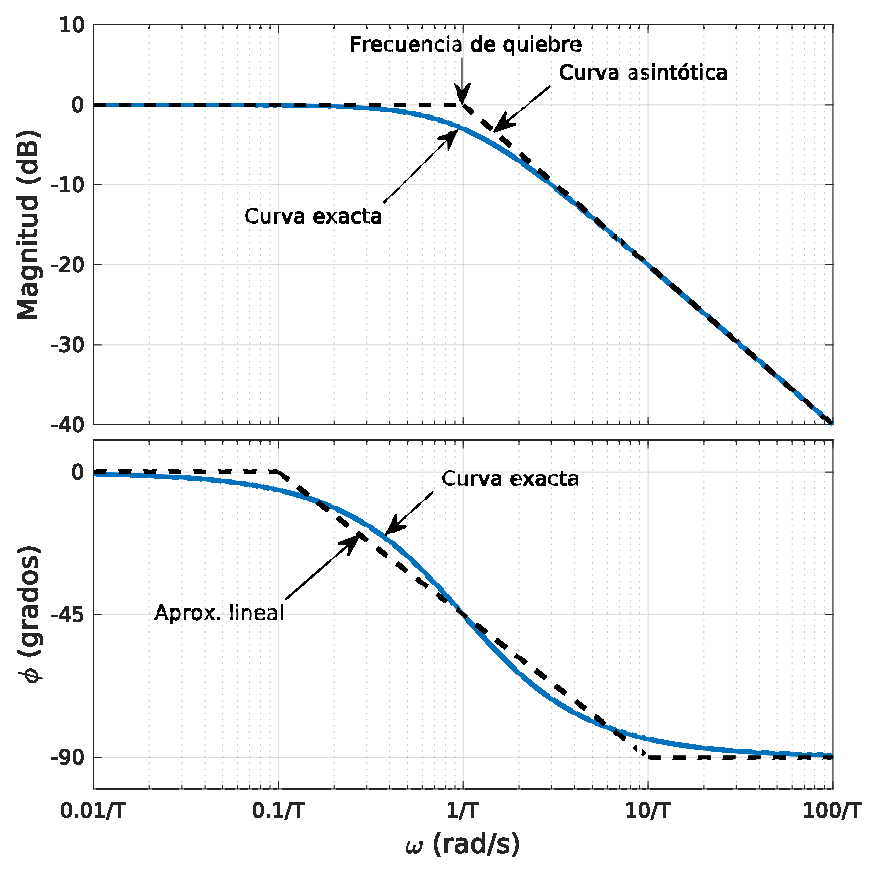
\includegraphics[width=6.5cm]{images/bodeFirstOrderIntegral.eps}
	\end{column}
\end{columns}
\end{frame}

\begin{frame}[<+->]\frametitle{Factores Básicos - Primer orden $(1+j \omega T)$}
\begin{columns}
	\begin{column}{0.5\textwidth}
	\small
	\begin{itemize}
		\item Magnitud: $\left| G(j\omega) \right| = 20 \log \left| 1+j\omega T \right|$
		\begin{equation*}
			\left| G(j\omega) \right| = 20 \log \sqrt{1+\omega^2 T^2}
		\end{equation*}
		\item Para bajas frecuencias ($\omega << 1/T$):
		\begin{equation*}
			\left| G(j\omega) \right| = 20 \log 1 = 0 \text{ dB}
		\end{equation*}
		\item Para altas frecuencias ($\omega >> 1/T$):
		\begin{equation*}
			\left| G(j\omega) \right| = 20 \log \omega T \text{ dB}
		\end{equation*}
		\item En la frecuencia de quiebre ($\omega = 1/T$):
		\begin{equation*}
			\left| G(j/T) \right| = 20\log \sqrt{1 + \frac{T^2}{T^2}} = 3.03 \text{ dB}
		\end{equation*}
	\end{itemize}
	\end{column}
	\begin{column}{0.5\textwidth}
	\centering
	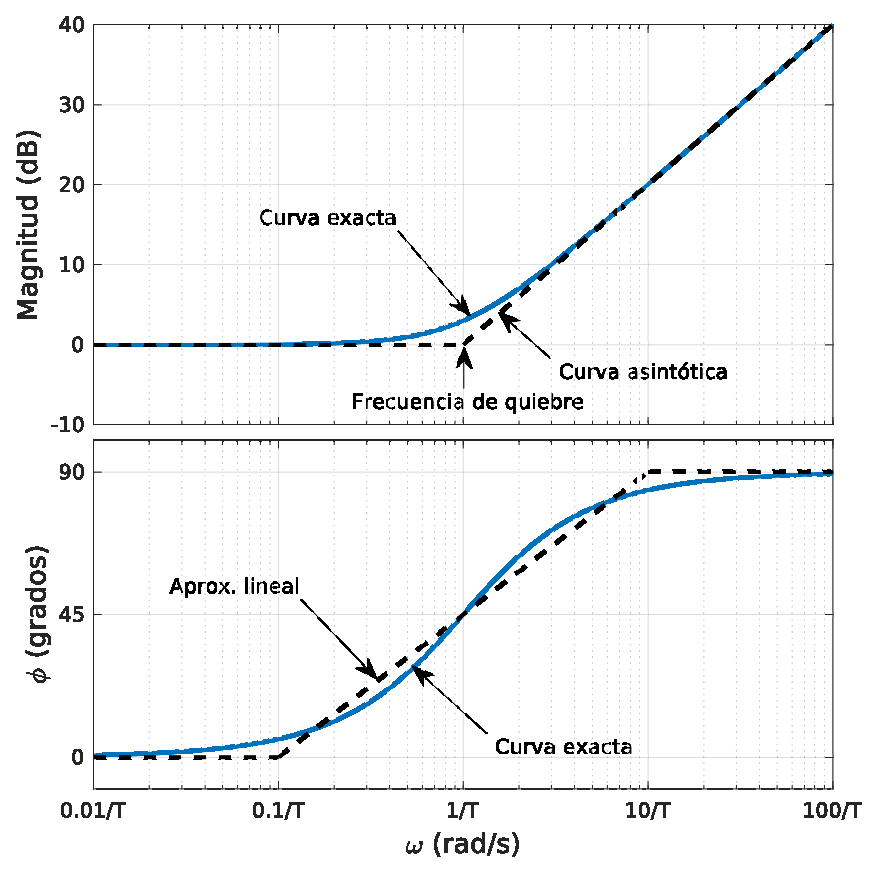
\includegraphics[width=6.5cm]{images/bodeFirstOrderDerivative.eps}
	\end{column}
\end{columns}
\end{frame}

\begin{frame}[<+->]\frametitle{Factores Básicos - Primer orden $(1+j \omega T)$}
\vspace*{8mm}
\begin{columns}
	\begin{column}{0.5\textwidth}
	\small
	\begin{itemize}
		\item Ángulo de fase: $\phi = \tan^{-1} \omega T$
		\item Para diferentes frecuencias:
		\begin{align*}
			\omega = 0 \hspace*{3mm} &\Rightarrow \hspace*{3mm} \phi = \tan^{-1} 0 = \ang{0}\\
			\omega = \frac{1}{T} \hspace*{3mm} &\Rightarrow \hspace*{3mm} \phi = \tan^{-1}\frac{T}{T} = \ang{45}\\
			\omega = \infty \hspace*{3mm} &\Rightarrow \hspace*{3mm} \phi =  \tan^{-1} \infty = \ang{90}
		\end{align*}
	\end{itemize}
	\end{column}
	\begin{column}{0.5\textwidth}
	\centering
	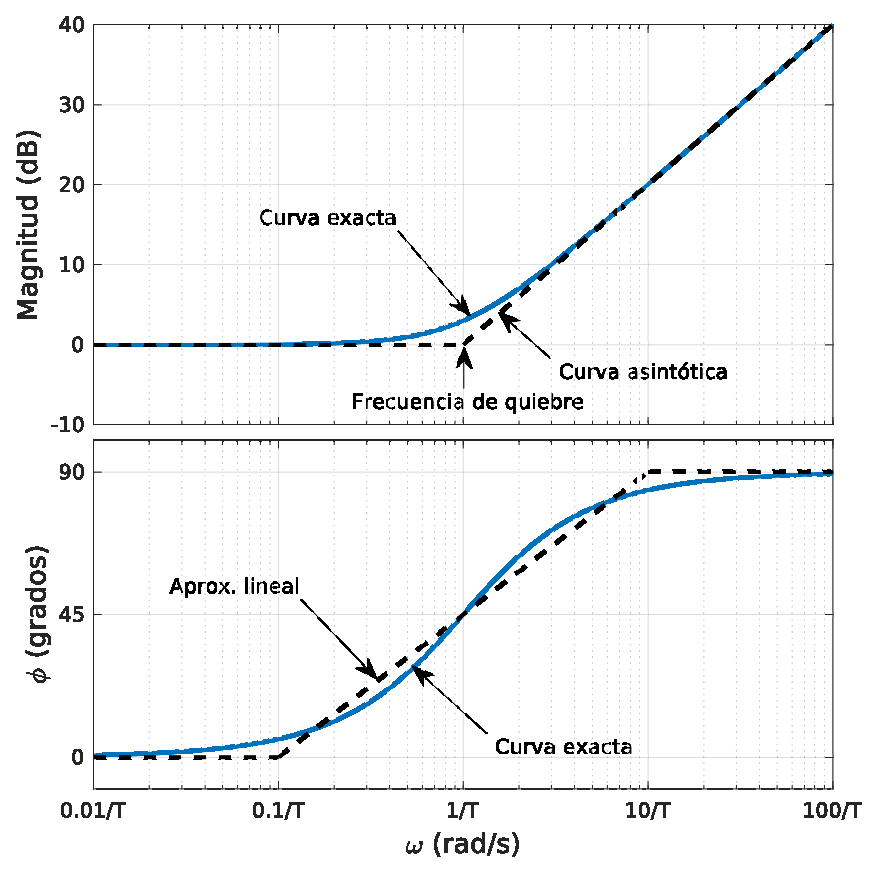
\includegraphics[width=6.5cm]{images/bodeFirstOrderDerivative.eps}
	\end{column}
\end{columns}
\end{frame}

\begin{frame}[<+->]\frametitle{Factores Básicos - Segundo orden $1/(1+2\zeta(j\omega/\omega_n)+(j\omega/\omega_n)^2)$}
\begin{columns}
	\begin{column}{0.5\textwidth}
	\begin{itemize}
		\item Magnitud:
		\begin{align*}
			\left| G(j\omega) \right| &= 20 \log \left| \frac{1}{1+2\zeta(j\omega/\omega_n)+(j\omega/\omega_n)^2} \right|\\
			&= -20 \log \sqrt{\left(1-\frac{\omega^2}{\omega_n^2}\right)^2+\left(2\zeta\frac{\omega}{\omega_n}\right)^2}
		\end{align*}
		\item Para bajas frecuencias ($\omega << \omega_n$):
		\begin{equation*}
			\left| G(j\omega) \right| = -20 \log 1 = 0 \text{ dB}
		\end{equation*}
		\item Para altas frecuencias ($\omega >> \omega_n$):
		\begin{equation*}
			\left| G(j\omega) \right| = -20 \log \frac{\omega^2}{\omega_n^2} = -40 \log \frac{\omega}{\omega_n} \text{ dB}
		\end{equation*}
	\end{itemize}
	\end{column}
	\begin{column}{0.5\textwidth}
	\centering
	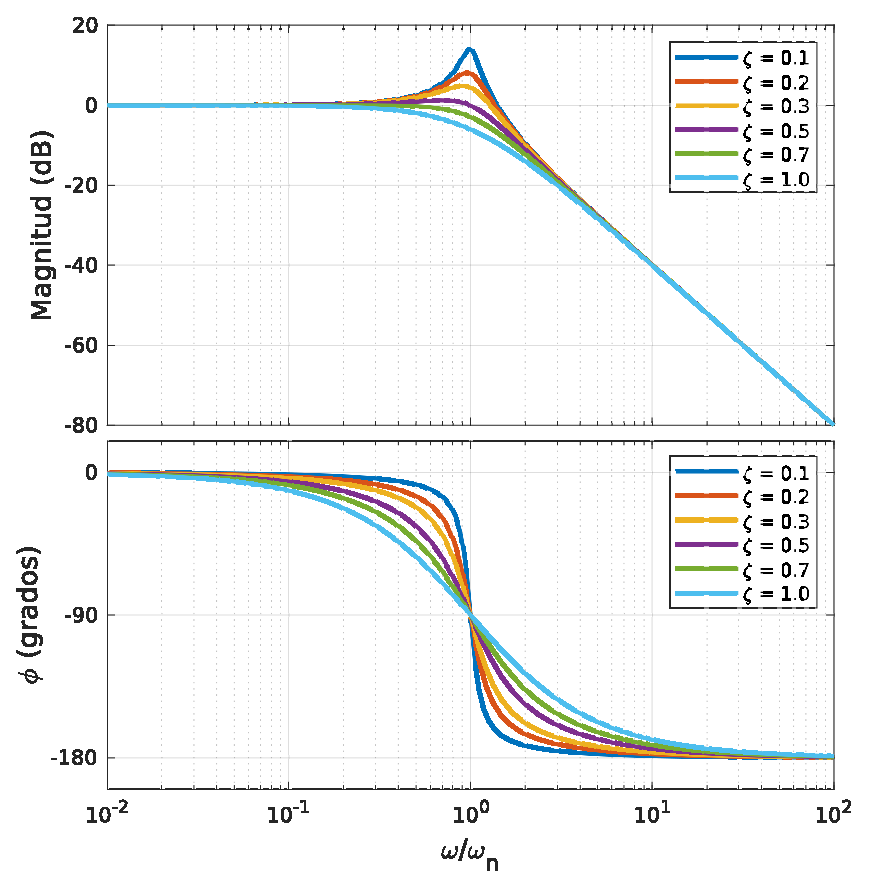
\includegraphics[width=6.5cm]{images/bodeSecondOrderIntegral.eps}
	\end{column}
\end{columns}
\end{frame}

\begin{frame}[<+->]\frametitle{Factores Básicos - Segundo orden $1/(1+2\zeta(j\omega/\omega_n)+(j\omega/\omega_n)^2)$}
\vspace*{7mm}
\begin{columns}
	\begin{column}{0.5\textwidth}
	\begin{itemize}
		\item Ángulo de fase:
		\begin{equation*}
			\angle G(j\omega) = -\tan^{-1} \left[\frac{2\zeta\frac{\omega}{\omega_n}}{1-\left(\frac{\omega}{\omega_n}\right)^2} \right]
		\end{equation*}
		\item En la frecuencia de quiebre $(\omega = \omega_n)$:
		\begin{equation*}
			\phi = -\tan^{-1}\left(\frac{2\zeta}{0}\right) = -\tan^{-1}\infty = -\ang{90}
		\end{equation*}
	\end{itemize}
	\end{column}
	\begin{column}{0.5\textwidth}
	\centering
	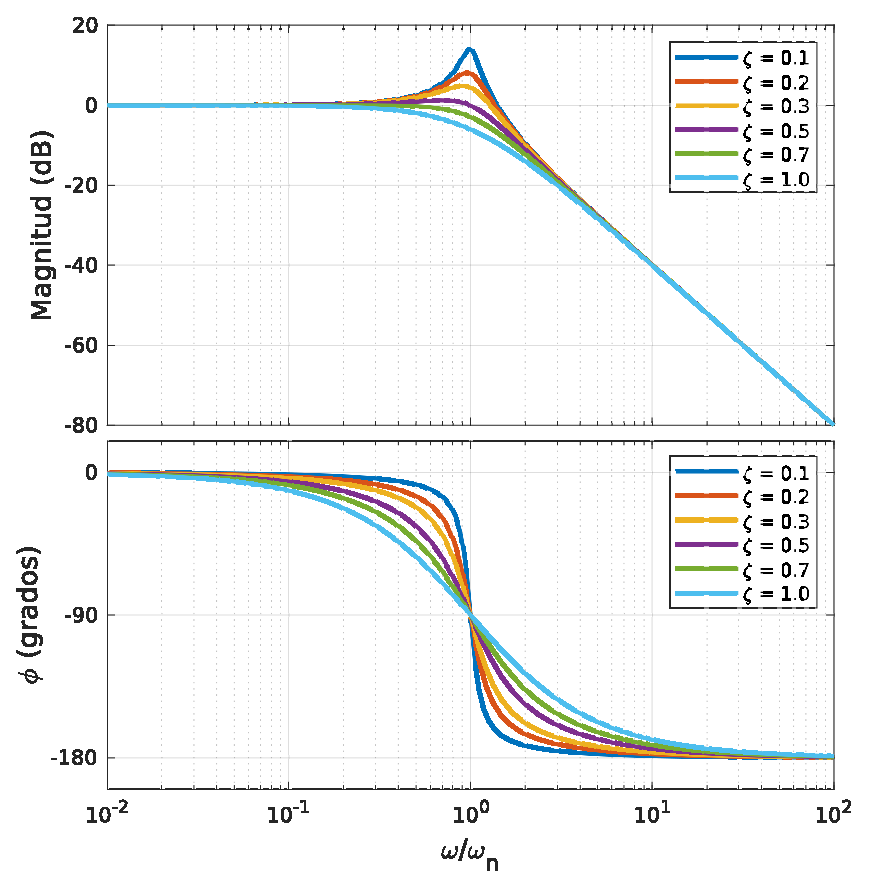
\includegraphics[width=6.5cm]{images/bodeSecondOrderIntegral.eps}
	\end{column}
\end{columns}
\end{frame}

\begin{frame}[<+->]\frametitle{Factores Básicos - Segundo orden $(1+2\zeta(j\omega/\omega_n)+(j\omega/\omega_n)^2)$}
\begin{columns}
	\begin{column}{0.5\textwidth}
	\begin{itemize}
		\item Magnitud:
		\begin{align*}
			\left| G(j\omega) \right| &= 20 \log \left| 1+2\zeta(j\omega/\omega_n)+(j\omega/\omega_n)^2 \right|\\
			&= 20 \log \sqrt{\left(1-\frac{\omega^2}{\omega_n^2}\right)^2+\left(2\zeta\frac{\omega}{\omega_n}\right)^2}
		\end{align*}
		\item Para bajas frecuencias ($\omega << \omega_n$):
		\begin{equation*}
			\left| G(j\omega) \right| = 20 \log 1 = 0 \text{ dB}
		\end{equation*}
		\item Para altas frecuencias ($\omega >> \omega_n$):
		\begin{equation*}
			\left| G(j\omega) \right| = 20 \log \frac{\omega^2}{\omega_n^2} = 40 \log \frac{\omega}{\omega_n} \text{ dB}
		\end{equation*}
	\end{itemize}
	\end{column}
	\begin{column}{0.5\textwidth}
	\centering
	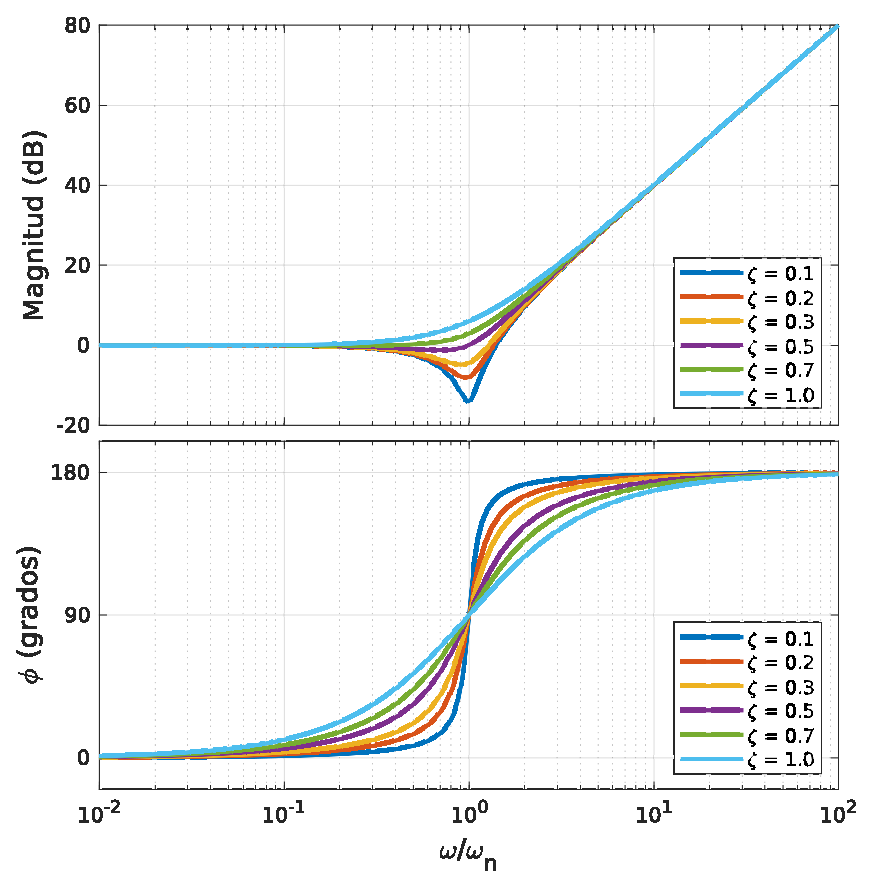
\includegraphics[width=6.5cm]{images/bodeSecondOrderDerivative.eps}
	\end{column}
\end{columns}
\end{frame}

\begin{frame}[<+->]\frametitle{Factores Básicos - Segundo orden $(1+2\zeta(j\omega/\omega_n)+(j\omega/\omega_n)^2)$}
\vspace*{7mm}
\begin{columns}
	\begin{column}{0.5\textwidth}
	\begin{itemize}
		\item Ángulo de fase:
		\begin{equation*}
			\angle G(j\omega) = \tan^{-1} \left[\frac{2\zeta\frac{\omega}{\omega_n}}{1-\left(\frac{\omega}{\omega_n}\right)^2} \right]
		\end{equation*}
		\item En la frecuencia de quiebre $(\omega = \omega_n)$:
		\begin{equation*}
			\phi = \tan^{-1}\left(\frac{2\zeta}{0}\right) = \tan^{-1}\infty = \ang{90}
		\end{equation*}
	\end{itemize}
	\end{column}
	\begin{column}{0.5\textwidth}
	\centering
	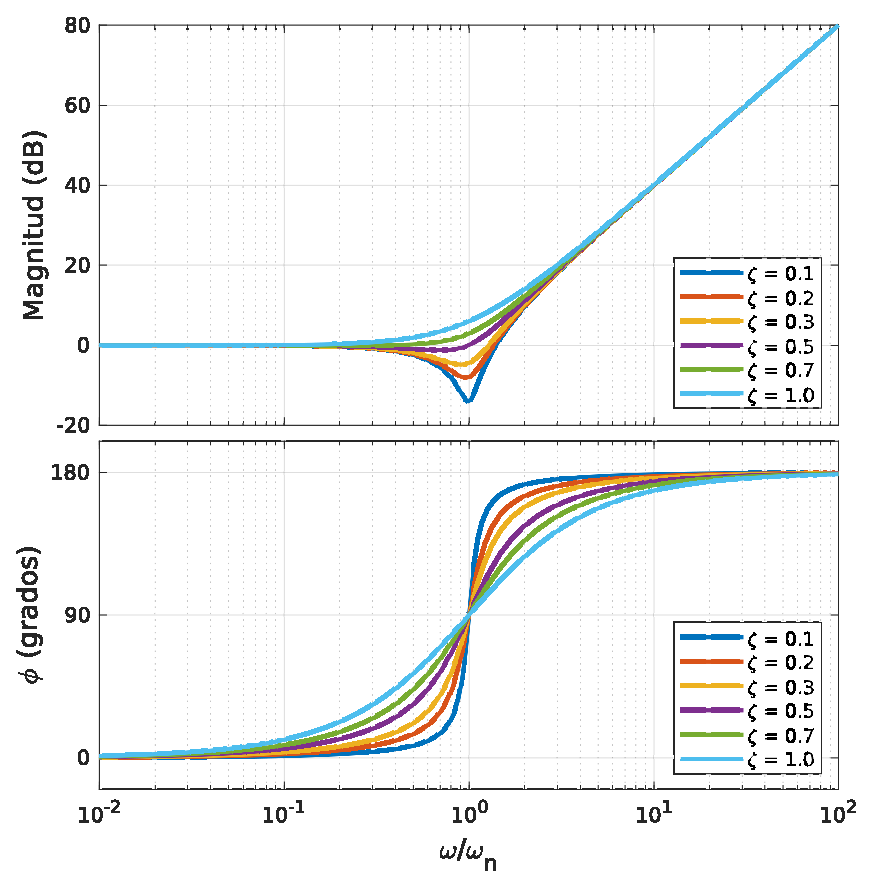
\includegraphics[width=6.5cm]{images/bodeSecondOrderDerivative.eps}
	\end{column}
\end{columns}
\end{frame}

\begin{frame}[<+->]\frametitle{Procedimiento para Obtener Diagramas de Bode}
	\begin{enumerate}
		\item Escribir la función de transferencia como un producto de factores básicos, en forma normalizada.
		\item Identificar las frecuencias de quiebre asociadas a cada uno de los factores.
		\item Dibujar las aproximaciones asintóticas de magnitud y fase con sus pendientes apropiadas.
		\item Sumar los segmentos para obtener la aproximación de la curva.
		\item Realizar las correcciones necesarias en los puntos de interés.
	\end{enumerate}
\end{frame}

\begin{frame}[<+->]\frametitle{Diagramas de Bode - Ejemplo}
	Dibuje el diagrama de bode para la siguiente función de transferencia:
	\begin{equation*}
		G(j\omega) = \frac{5(1+j0.1\omega)}{j\omega(1+j0.5\omega)[1+j0.6(\omega/50)+(j\omega/50)^2]}
	\end{equation*}
	\pause
	Los factores presentes en la función de transferencia son:
	\begin{enumerate}
		\item Una ganancia constante: $G_1(j\omega) = 5$
		\item Un polo en el origen: $G_2(j\omega) = (j\omega)^{-1}$
		\item Un polo en $\omega = 2$: $G_3(j\omega) = \left(1+j\frac{\omega}{2}\right)^{-1}$
		\item Un cero en $\omega = 10$: $G_4(j\omega) = 1+j\frac{\omega}{10}$
		\item Un par de polos complejos en $\omega = 50$: $G_5(j\omega) = 1+j0.6\omega/50+(j\omega/50)^2$
	\end{enumerate}
\end{frame}

\begin{frame}[<+->]\frametitle{Diagramas de Bode - Ejemplo}
	\vspace*{-2mm}
	\begin{columns}
		\begin{column}{0.3\textwidth}
			Aproximaciones asintóticas de magnitud y fase de cada factor (líneas sólidas) y curvas exactas (líneas punteadas).
		\end{column}
		\begin{column}{0.7\textwidth}
	\begin{figure}
		\centering
		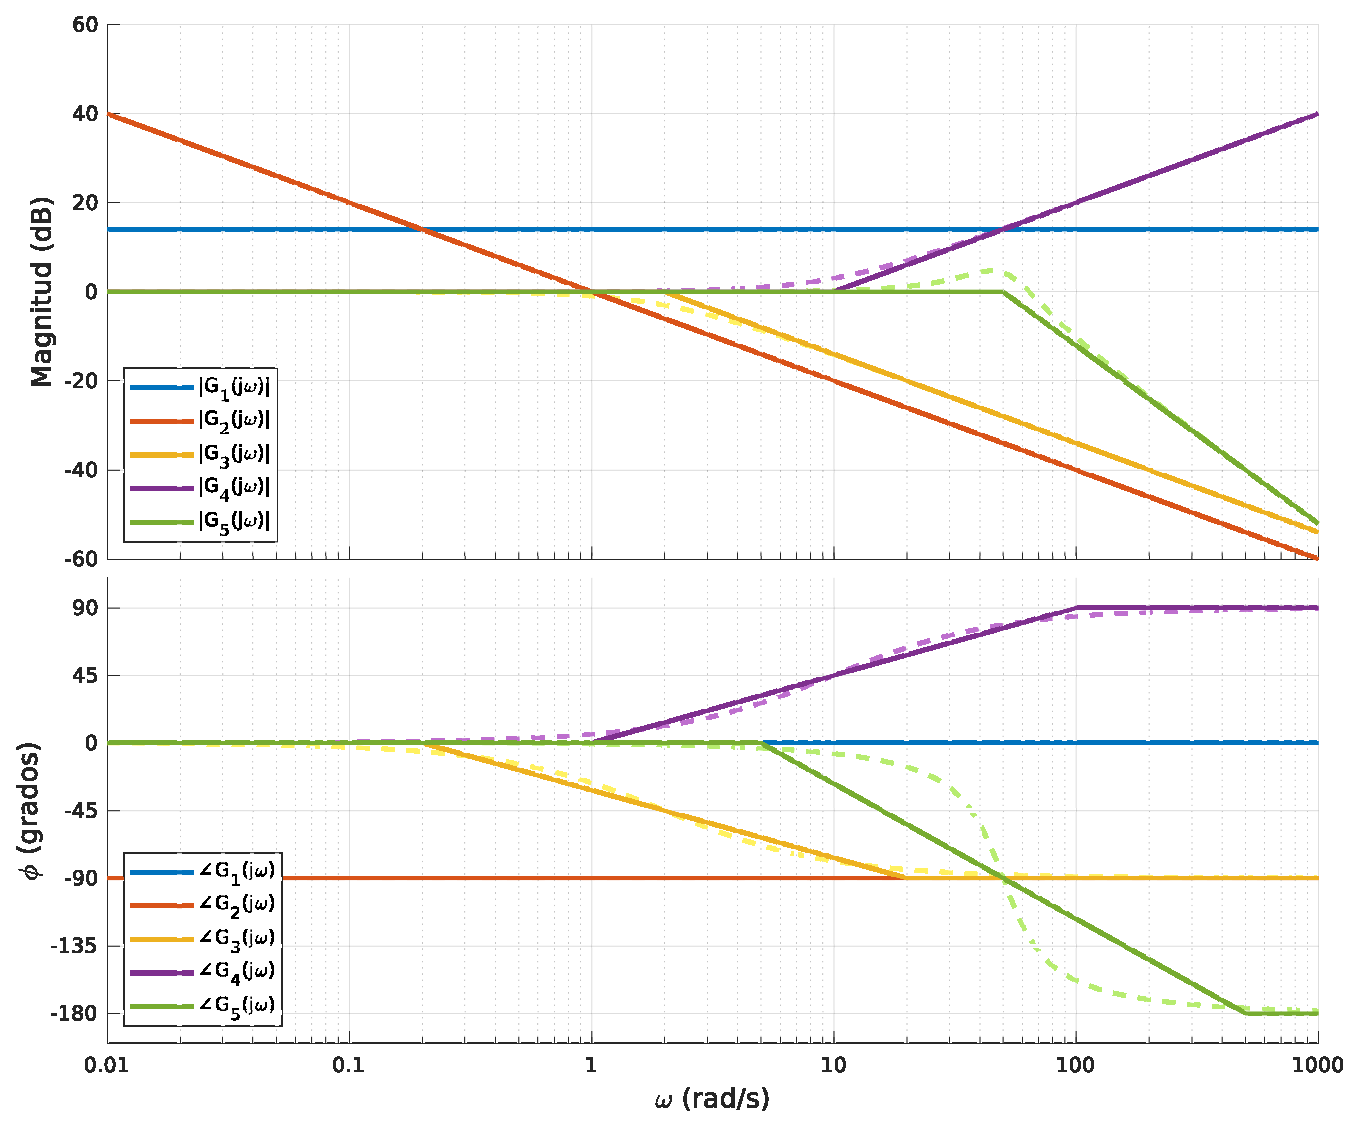
\includegraphics[width=9cm]{images/bodeExample1a.eps}
	\end{figure}
		\end{column}
	\end{columns}
\end{frame}

\begin{frame}[<+->]\frametitle{Diagramas de Bode - Ejemplo}
	\vspace*{-2mm}
	\begin{columns}
		\begin{column}{0.3\textwidth}
			Sumando las asíntotas obtenidas para cada factor se obtiene una aproximación de los diagramas exactos de magnitud y fase.
		\end{column}
		\begin{column}{0.7\textwidth}
			\begin{figure}
				\centering
				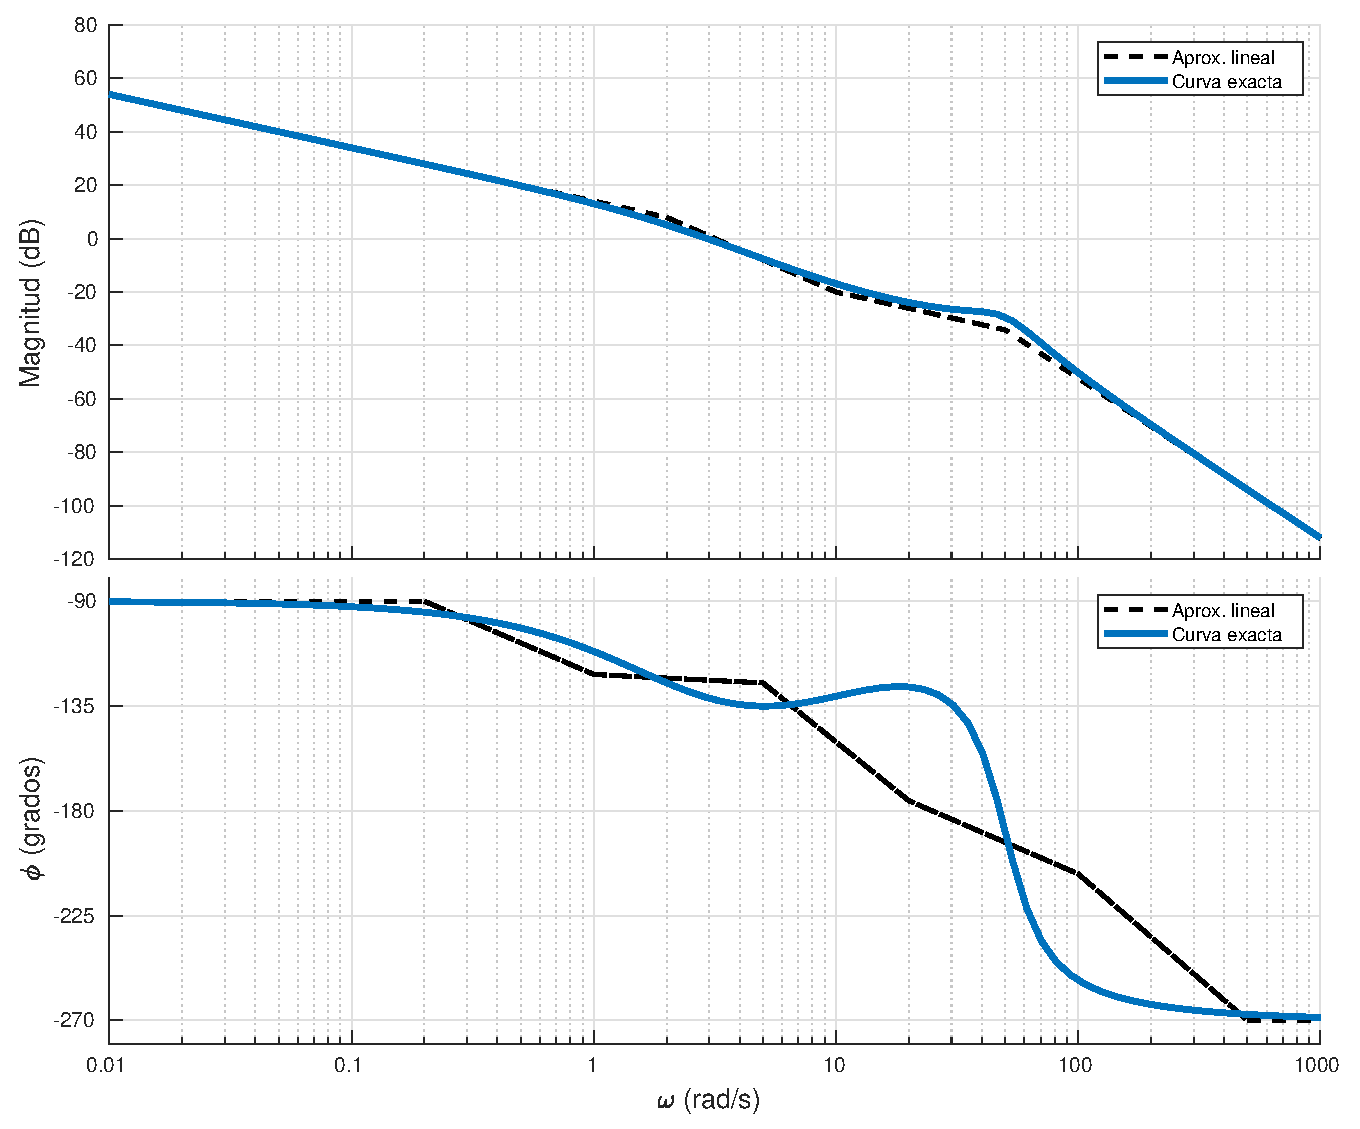
\includegraphics[width=9cm]{images/bodeExample1b.eps}
			\end{figure}
		\end{column}
	\end{columns}
\end{frame}

\begin{frame}[<+->]\frametitle{Márgenes de Estabilidad}
	\begin{columns}
		\begin{column}{0.45\textwidth}
			\begin{itemize}
				\item Frecuencia de cruce de ganancia: Frecuencia a la cual la ganancia del sistema se hace unitaria:
				\begin{equation*}
					20 \log |G(j\omega_{cg})| = 0 \text{ dB}
				\end{equation*}
				\item Frecuencia de cruce de fase: Frecuencia a la cual la fase del sistema se hace \ang{180}:
				\begin{equation*}
					\angle G(j\omega_{cp}) = \ang{180}
				\end{equation*}
			\end{itemize}
		\end{column}
		\begin{column}{0.55\textwidth}
		\begin{figure}
			\centering
			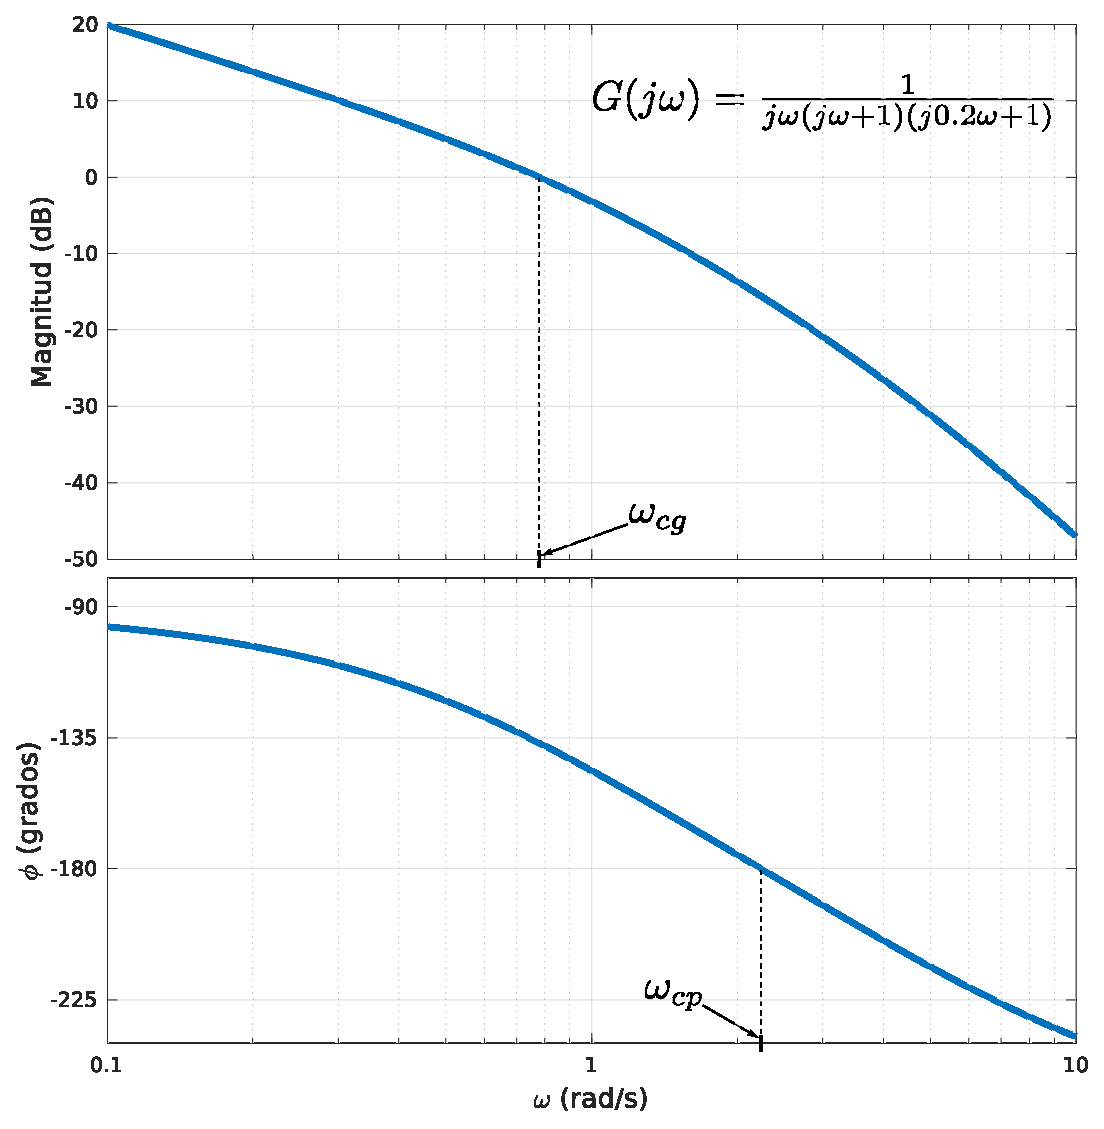
\includegraphics[width=7cm]{images/phaseGainCutFreqExample.eps}
		\end{figure}
		\end{column}
	\end{columns}	
\end{frame}

\begin{frame}[<+->]\frametitle{Márgenes de Estabilidad}
	\small
	\begin{columns}
		\begin{column}{0.45\textwidth}
			\begin{itemize}
				\item Margen de Fase: Fase faltante en la frecuencia de cruce de ganancia $\omega_{cg}$ para que el sistema en lazo cerrado se encuentre al borde de la inestabilidad:
				\begin{equation*}
					PM = \ang{180} - \angle G(j\omega_{cg})
				\end{equation*}
				\item Margen de Ganancia: Ganancia en la frecuencia de cruce de fase $\omega_{cp}$ para que el sistema en lazo cerrado se encuentre al borde de la inestabilidad:
				\begin{equation*}
					GM = \frac{1}{|G(j\omega_{cp})|}
				\end{equation*}
			\end{itemize}
		\end{column}
		\begin{column}{0.55\textwidth}
		\begin{figure}
			\vspace*{-4mm}
			\centering
			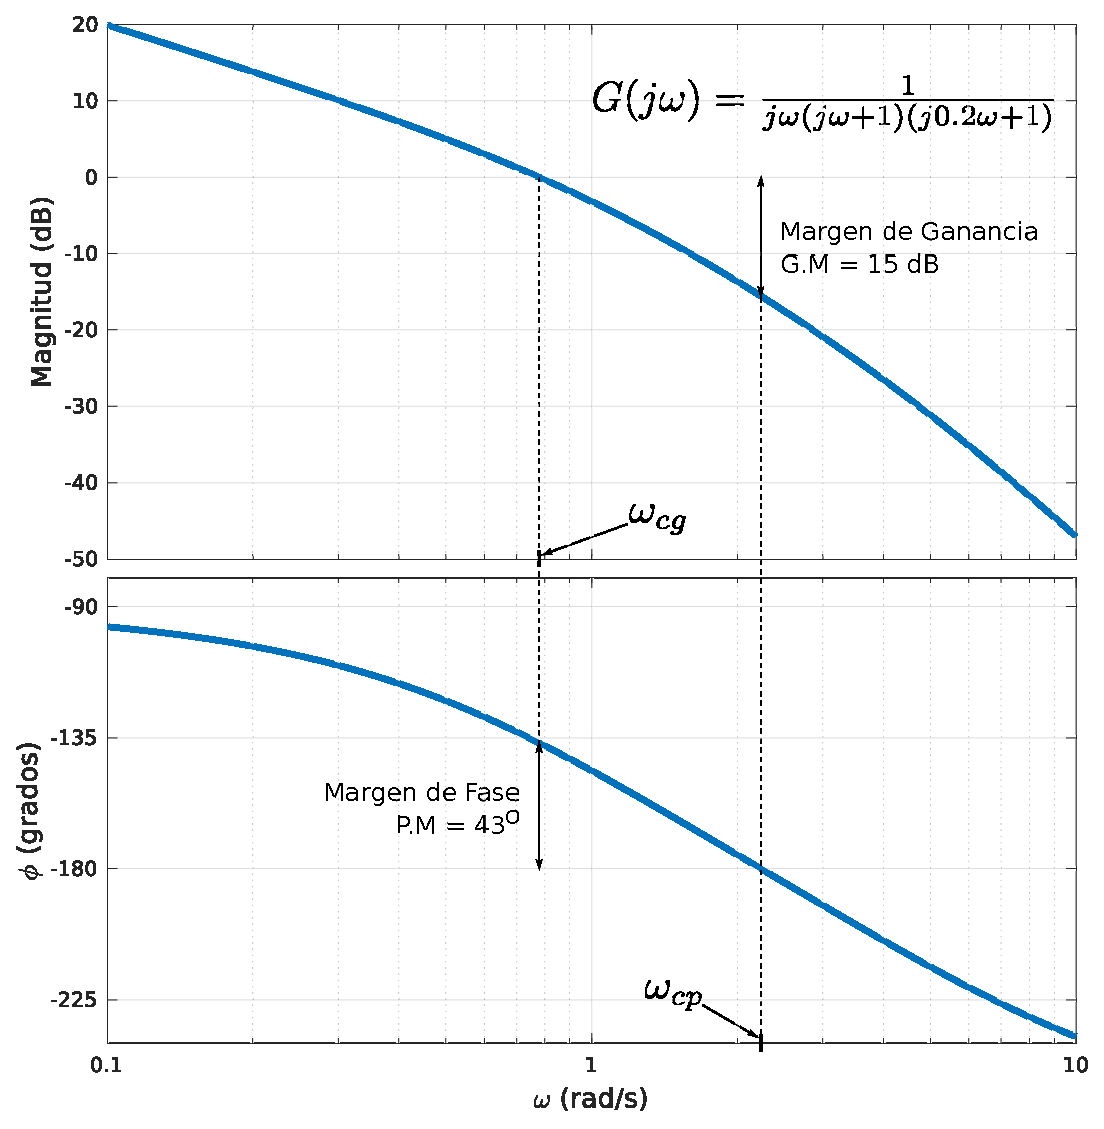
\includegraphics[width=7cm]{images/phaseGainMarginsExample.eps}
		\end{figure}
		\end{column}
	\end{columns}	
\end{frame}

\begin{frame}[<+->]\frametitle{Márgenes de Estabilidad}
	\begin{figure}
		\centering
		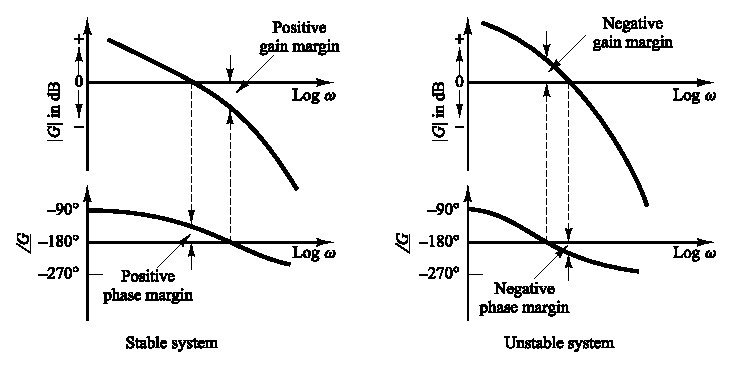
\includegraphics[width=9cm]{images/phaseGainMarginsStability.eps}
	\end{figure}
	\vspace*{-3mm}
	\begin{itemize}
		\item Para un sistema de fase mínima (función de transferencia de lazo abierto sin ceros ni polos en el semiplano derecho):
		\begin{itemize}
			\item Tanto el margen de fase como de ganancia deben ser positivos para que el sistema sea estable.
			\item Márgenes de fase negativos indican inestabilidad.
		\end{itemize}
	\end{itemize}
\end{frame}

\begin{frame}[<+->]\frametitle{Características de la Respuesta en Frecuencia}
	\begin{itemize}
		\item Lugar de las raíces $\rightarrow$ útil para modificar la respuesta transitoria en el tiempo de sistemas de control en lazo cerrado.
		\item Respuesta en frecuencia:
		\begin{itemize}
			\item No provee directamente información sobre la respuesta transitoria. Sin embargo es útil para diseñar compensadores.
			\item Se especifica el desempeño de la respuesta transitoria de manera indirecta:
			\begin{itemize}
				\item Margen de fase / ganancia, pico de magnitud resonante $\rightarrow$ proveen un estimado del amortiguamiento.
				\item Frecuencia de cruce de ganancia, frecuencia de resonancia, ancho de banda $\rightarrow$ velocidad de la respuesta transitoria.
				\item Constantes de error estático $\rightarrow$ exactitud de la respuesta en estado estacionario.
			\end{itemize}
			\item Las especificaciones en frecuencia se pueden satisfacer usando el diagrama de Bode.
		\end{itemize}
	\end{itemize}
\end{frame}


\begin{frame}[<+->]\frametitle{Características de la Respuesta en Frecuencia}
\begin{itemize}
	\item Información obtenible a partir de la respuesta en frecuencia de lazo abierto:
	\begin{itemize}
		\item Bajas frecuencias ($\omega << \omega_{cg}$) $\rightarrow$ indica el comportamiento en estado estacionario en lazo cerrado del sistema.
		\item Medias frecuencias ($\omega \text{ cercano a } \omega_{cg}$) $\rightarrow$ indica la estabilidad relativa.
		\item Altas frecuencias ($\omega >> \omega_{cg}$) $\rightarrow$ indica la complejidad del sistema.
	\end{itemize}
	\item Requerimientos de la respuesta en frecuencia de lazo abierto:
	\begin{itemize}
		\item Compensación $\rightarrow$ balance entre la exactitud en estado estacionario y la estabilidad relativa.
		\item Ganancia en baja frecuencia: debería ser suficientemente alta.
		\item La pendiente debería ser de -20 dB cerca a $\omega_{cg}$ y extenderse en una banda de frecuencia suficiente para garantizar un MF apropiado.
		\item La ganancia en alta frecuencia debería atenuarse rápidamente para minimizar los efectos del ruido.
	\end{itemize}
\end{itemize}
\end{frame}

\section{Compensación Usando la Respuesta en Frecuencia}
\begin{frame}[<+->]\frametitle{Compensadores - Características de los Diferentes Esquemas de Compensación}
 	\begin{itemize}
 		\item Compensación en adelanto:
 		\begin{itemize}
 			\item Ofrece una mejora notable en la respuesta transitoria con un pequeño cambio en la exactitud de estado estacionario.
 			\item Puede acentuar efectos de ruido de alta frecuencia.
 			\item Aumenta el orden del sistema en 1 (a menos que exista cancelación polo-cero).
 		\end{itemize}
 		\item Compensación en atraso:
 		\begin{itemize}
 			\item Ofrece una mejora notable en la exactitud de estado estacionario, pero aumentando el tiempo de la respuesta transitoria.
 			\item Elimina los efectos de señales de ruido de alta frecuencia.
 			\item Aumenta el orden del sistema en 1 (a menos que exista cancelación polo-cero).
 		\end{itemize}
 		\item Compensación adelanto-atraso:
 		\begin{itemize}
 			\item Combina las características de los dos tipos de compensación.
 			\item Aumenta el orden del sistema en 2 (a menos que exista cancelación polo-cero).
 			\item El sistema se hace más complejo y es más difícil controlar la respuesta transitoria.
 		\end{itemize}
  \end{itemize}    
\end{frame}

\begin{frame}[<+->]\frametitle{Compensador en Adelanto}
	\begin{equation*}
		G_c(s) = K_c \alpha \frac{T s + 1}{\alpha T s + 1} = K_c \frac{s+\frac{1}{T}}{s + \frac{1}{\alpha T}}\hspace*{6mm} (0 < \alpha < 1)
	\end{equation*}
	\pause
	\begin{itemize}
		\item $\alpha$: Factor de atenuación del compensador.
		\item El compensador tiene un cero en $s = -1/T$ y un polo en $s = -1/\alpha T$.
		\item Dado que $0 < \alpha < 1$ $\Rightarrow$ el cero se ubica a la derecha del polo.
		\item Para $\alpha$ muy pequeño $\Rightarrow$ el polo se localiza lejos hacia la izquierda.
		\item Usualmente el valor mínimo de $\alpha$ es 0.05 $\Rightarrow$ máximo adelanto de fase es cercano a \ang{65}. 
	\end{itemize}
\end{frame}

\begin{frame}[<+->]\frametitle{Compensador en Adelanto}
\vspace*{3mm}
\begin{columns}
	\begin{column}{0.5\textwidth}
		Reemplazando $s=j\omega$ y graficando $Re\left\{G(j\omega)\right\}$ vs. $Im\left\{G(j\omega)\right\}$ para $K_c=1$:
		\begin{equation*}
			G_c(j\omega) = K_c \alpha \frac{j\omega T + 1}{j\omega \alpha T + 1}
		\end{equation*}
		\begin{figure}
			\centering 
			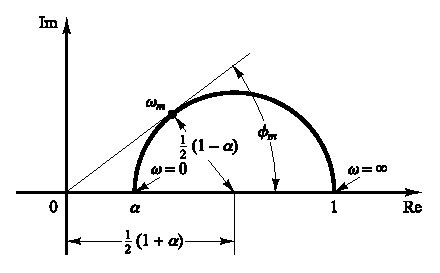
\includegraphics[width=5cm]{images/polarPlot.eps}
		\end{figure}
	\end{column}
	\begin{column}{0.5\textwidth}
		\begin{itemize}
			\item $\phi_m$: máximo ángulo de adelanto de fase.
			\item $\omega_m$: frecuencia en el punto tangente.
			\item De la figura se obtiene:
			\begin{equation*}
				\sin \phi_m = \frac{\frac{1-\alpha}{2}}{\frac{1+\alpha}{2}} = \frac{1-\alpha}{1+\alpha}
			\end{equation*}
		\end{itemize}
	\end{column}
\end{columns}
\end{frame}

\begin{frame}[<+->]\frametitle{Compensador en Adelanto}
\begin{columns}
	\begin{column}{0.5\textwidth}
	Diagrama de bode del compensador para $K_c=1$, $\alpha=0.1$.
	\begin{itemize}
		\item Frecuencias de quiebre: $\omega = 1/T$, $\omega = 1/\alpha T$.
		\item Media geométrica de las frecuencias de quiebre:
		\begin{align*}
			\log \omega_m &=\frac{1}{2}\left( \log \frac{1}{T} + \log \frac{1}{\alpha T} \right)\\
			\omega_m &= \frac{1}{\sqrt{\alpha}T}
		\end{align*}
	\end{itemize}
	\end{column}
	\begin{column}{0.5\textwidth}
	\begin{figure}
		\centering
		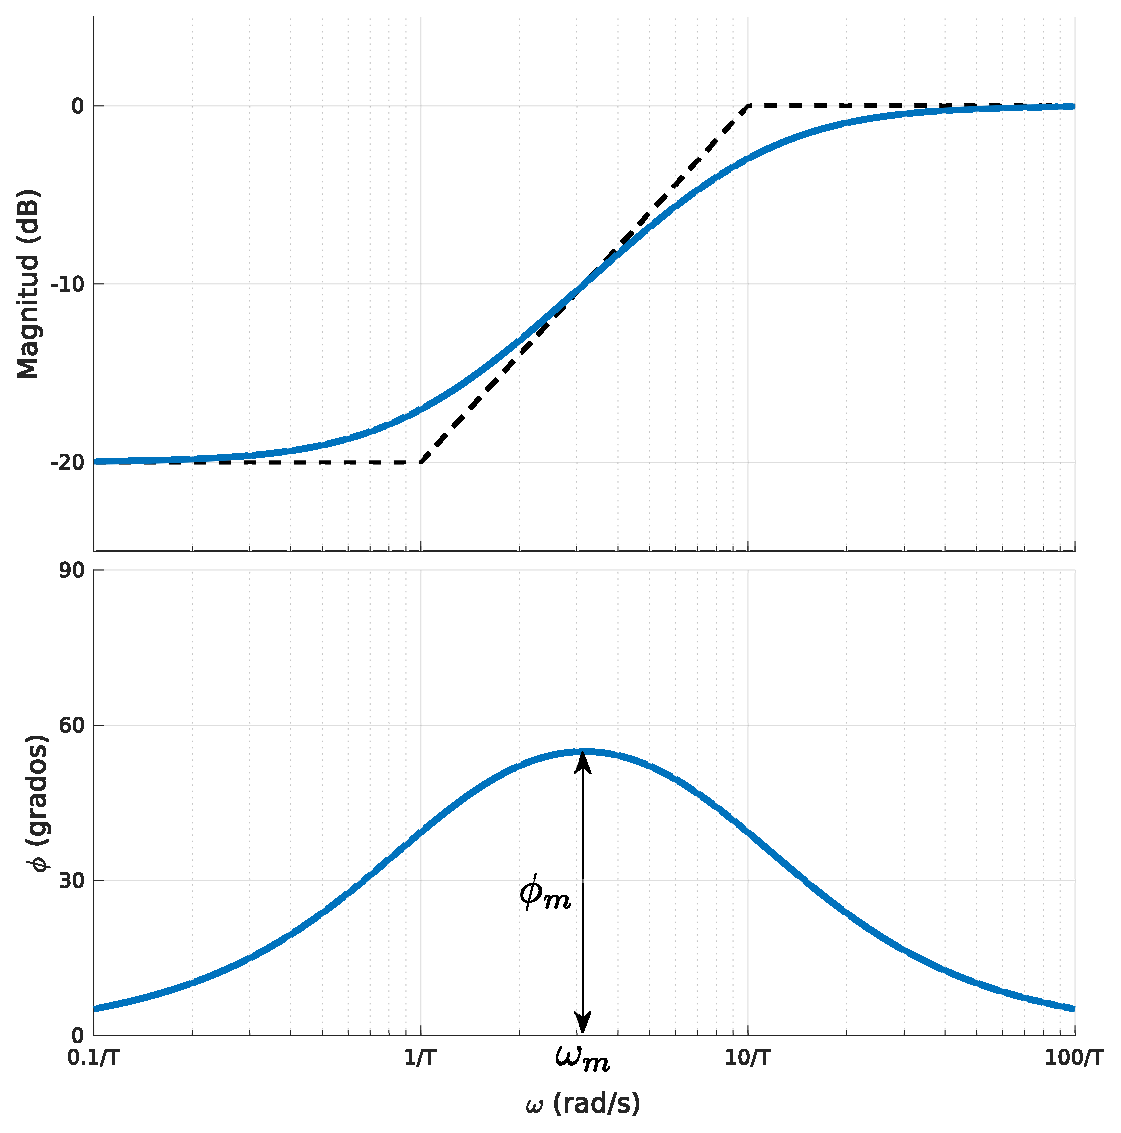
\includegraphics[width=7cm]{images/bodeLeadComp.eps}
	\end{figure}
	\end{column}
\end{columns}
\end{frame}

\begin{frame}[<+->]\frametitle{Compensador en Adelanto: Procedimiento de Diseño}
	\begin{enumerate}
		\item Se asume la siguiente forma para el compensador en adelanto:
		\begin{equation*}
			G_c(s) = K_c \alpha \frac{Ts+1}{\alpha Ts+1} = K_c \frac{s+\frac{1}{T}}{s+\frac{1}{\alpha T}}, \hspace*{3mm} (0 < \alpha < 1)
		\end{equation*}
		\pause
		Definiendo $K_c \alpha = K$, se tiene
		\begin{equation*}
			G_c(s) = K \frac{Ts+1}{\alpha Ts+1}
		\end{equation*}
		\pause
		La F.T. de lazo abierto del sistema compensado es:
		\begin{equation*}
			G_c(s)G(s) = K \frac{Ts+1}{\alpha Ts+1}G(s) = \frac{Ts+1}{\alpha Ts+1} KG(s) = \frac{Ts+1}{\alpha Ts+1} G_1(s)
		\end{equation*}
		donde $G_1(s) = KG(s)$.
		\pause
		Determinar $K$ para satisfacer el requerimiento dado por la constante de error estático.
		\seti
	\end{enumerate}
\end{frame}

\begin{frame}[<+->]\frametitle{Compensador en Adelanto: Procedimiento de Diseño}
	\begin{enumerate}
		\conti
		\item Usando la ganancia $K$ determinada, dibujar el diagrama de Bode del sistema $G_1(s)$. Evaluar el margen de fase.
		\item Determinar el ángulo de adelanto de fase requerido, agregando un ángulo adicional de \ang{5} a \ang{12} debido a que el compensador de adelanto desplaza la frecuencia de cruce de ganancia hacia la derecha, disminuyendo el margen de fase.
		\item Determinar el factor de atenuación $\alpha$ usando la ecuación
		\begin{equation*}
			\sin \phi_m = \frac{1-\alpha}{1+\alpha}
		\end{equation*}
		Determinar la nueva frecuencia de cruce de ganancia como $\omega_m = 1/(\sqrt{\alpha}T)$.
		\seti
	\end{enumerate}
\end{frame}

\begin{frame}[<+->]\frametitle{Compensador en Adelanto: Procedimiento de Diseño}
	\begin{enumerate}
		\conti
		\item Determinar las frecuencias de quiebre del compensador como:
		\begin{itemize}
			\item Cero: $\omega = 1/T$.
			\item Polo: $\omega = 1/(\alpha T)$.
		\end{itemize}
		\item Usando los valores de $K$ y $\alpha$ calcular $K_c = K/\alpha$.
		\item Verificar el margen de ganancia para asegurarse que sea satisfactorio. En caso contrario, repetir el proceso modificando la ubicación polo-cero del compensador hasta lograr un resultado satisfactorio.
		\seti
	\end{enumerate}
\end{frame}

\begin{frame}[<+->]\frametitle{Compensador en Adelanto: Ejemplo}
	Considere el sistema $G(s) = \frac{4}{s(s+2)}$ con retroalimentación unitaria:
	\begin{figure}
		\centering
		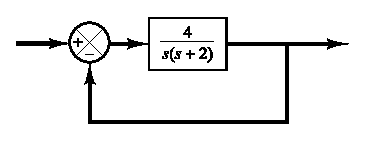
\includegraphics[width=4cm]{images/leadCompExampleSystem.eps}
	\end{figure}
	Se desea diseñar un compensador para que el sistema tenga una constante de error estático de velocidad $K_v = 20$, margen de fase de al menos \ang{50} y margen de ganancia de al menos 10 dB.
\end{frame}

\begin{frame}[<+->]\frametitle{Compensador en Adelanto: Ejemplo}
	En primer lugar se calcula $K$ para satisfacer el requerimiento de $K_v = 20$:
	\begin{align*}
		K_v &= \lim_{s\rightarrow 0} sG_c(s)G(s) = \lim_{s \rightarrow 0} s\frac{Ts+1}{\alpha T s + 1} \frac{4K}{s(s+2)} = 2K = 20\\
		&\Rightarrow K = 10
	\end{align*}
	\pause
	Entonces, la función de transferencia del sistema $G_1(s)$ queda:
	\begin{equation*}
		G_1(s) = \frac{40}{j\omega(j\omega+2)}
	\end{equation*}
\end{frame}

\begin{frame}[<+->]\frametitle{Compensador en Adelanto: Ejemplo}
	\vspace*{-7mm}
  \begin{columns}
  	\begin{column}{0.4\textwidth}
			Graficando el diagrama de Bode para $G_1(s)$ usando la función \texttt{margin} de Matlab se obtiene:
			\begin{align*}
				PM &= \ang{18}\\
				GM &= \infty
			\end{align*}
  	\end{column}
  	\begin{column}{0.6\textwidth}
			\begin{figure}
				\centering
				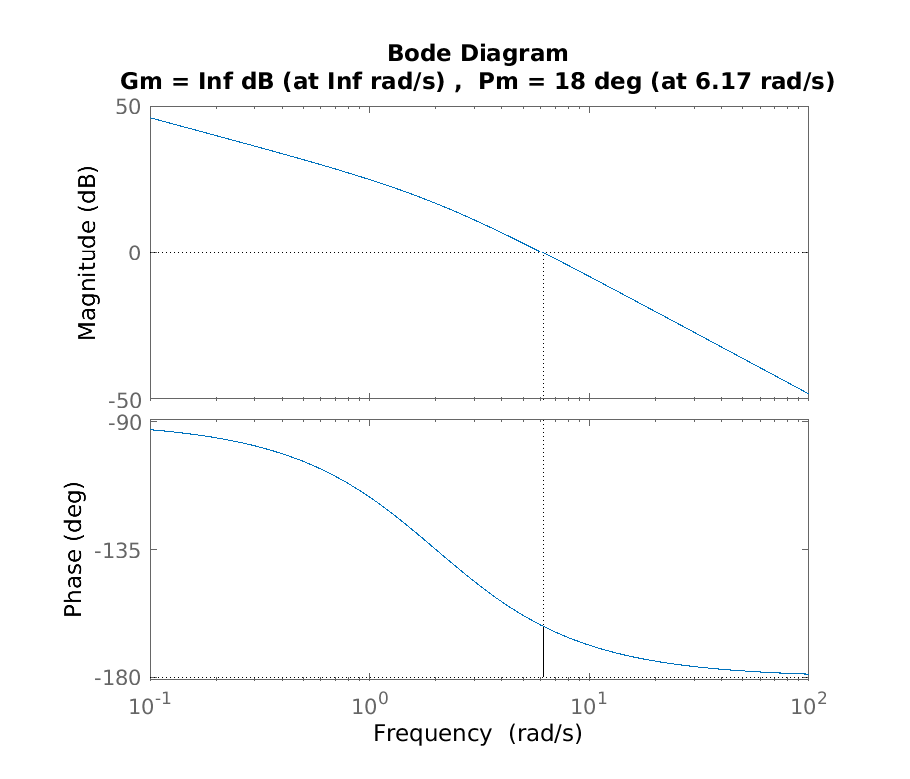
\includegraphics[width=8.5cm]{images/bodeLeadCompExample.eps} 	
		  \end{figure}
  	\end{column}
  \end{columns}
\end{frame}

\begin{frame}[<+->]\frametitle{Compensador en Adelanto: Ejemplo}   
	Para satisfacer $PM = \ang{50}$ se requiere que el compensador aporte un ángulo de adelanto de fase 
	\begin{equation*}
		\phi_m = \ang{50} - \ang{18} + \ang{5} = \ang{37}
	\end{equation*}
	Considerando el desplazamiento del diagrama debido al compensador, se agregó un ángulo adicional de \ang{5}.
\end{frame}

\begin{frame}[<+->]\frametitle{Compensador en Adelanto: Ejemplo}
\vspace*{5mm}
\begin{columns}
	\begin{column}{0.5\textwidth}		
	Dado que
	\begin{equation*}
		\sin \phi_m = \frac{1-\alpha}{1+\alpha}
	\end{equation*}
	un ángulo de adelanto de fase $\phi_m = \ang{37}$ corresponde a $\alpha = 0.2486$.
	\pause\\
	\vspace*{3mm}
	Para determinar las frecuencias de quiebre $\omega = \frac{1}{T}$ y $\omega = \frac{1}{\alpha T}$ se considera que el máximo adelanto de fase $\phi_m$ ocurre en la media geométrica de las dos frecuencias dada por $\omega = \frac{1}{\sqrt{\alpha}T}$.
	\pause
	\end{column}
	\begin{column}{0.5\textwidth}
	En esta frecuencia, el aporte de ganancia del compensador es:
	\begin{align*}
		&\left| \frac{1+j\omega T}{1 + j\omega \alpha T} \right|_{\omega = 1/(\sqrt{\alpha}T)} = \left| \frac{1+j\frac{1}{\sqrt{\alpha}}}{1+j\alpha\frac{1}{\sqrt{\alpha}}} \right|\\
		 &= \frac{1}{\sqrt{\alpha}} = 6.0453 \text{ dB}
	\end{align*}
	\end{column}
\end{columns}
\end{frame}

\begin{frame}[<+->]\frametitle{Compensador en Adelanto: Ejemplo}
\begin{columns}
	\begin{column}{0.5\textwidth}
	La frecuencia donde $|G_1(j\omega)| = -6.0453$ corresponde a 8.85 rad/s. Ésta se selecciona como la nueva frecuencia de corte de ganancia $\omega_{cg}$.
	\pause\\
	\vspace*{3mm}
	Dado que ésta frecuencia corresponde a $\omega_{cg} = \frac{1}{\sqrt{\alpha}T}$ entonces:
	\begin{equation*}
		 \frac{1}{T} = 4.9112,\hspace*{3mm} \frac{1}{\alpha T} = 20.1062
	\end{equation*}
	\pause
	\end{column}
	\begin{column}{0.5\textwidth}
	Por lo tanto el compensador corresponde a:
	\begin{equation*}
		G_c(s) = K_c\frac{s+4.9112}{s+20.1062} = K_c \alpha \frac{0.2036s + 1}{0.0497s + 1}
	\end{equation*}
	\pause\\
	El valor de $K_c$ se encuentra como $K_c = \frac{K}{\alpha} = \frac{10}{0.2486} = 40.2253$. Entonces, el compensador queda:
	\begin{equation*}
		G_c(s) = 10.0121 \frac{0.2036s + 1}{0.0497s + 1}
	\end{equation*}
	\end{column}
\end{columns}
\end{frame}

\begin{frame}[<+->]\frametitle{Compensador en Adelanto: Ejemplo - Diagrama de Bode}
\begin{columns}
	\begin{column}{0.3\textwidth}
		El sistema compensado tiene mayor ancho de banda y satisface el requerimiento de margen de fase.
	\end{column}
	\begin{column}{0.7\textwidth}
		\begin{figure}
			\centering
			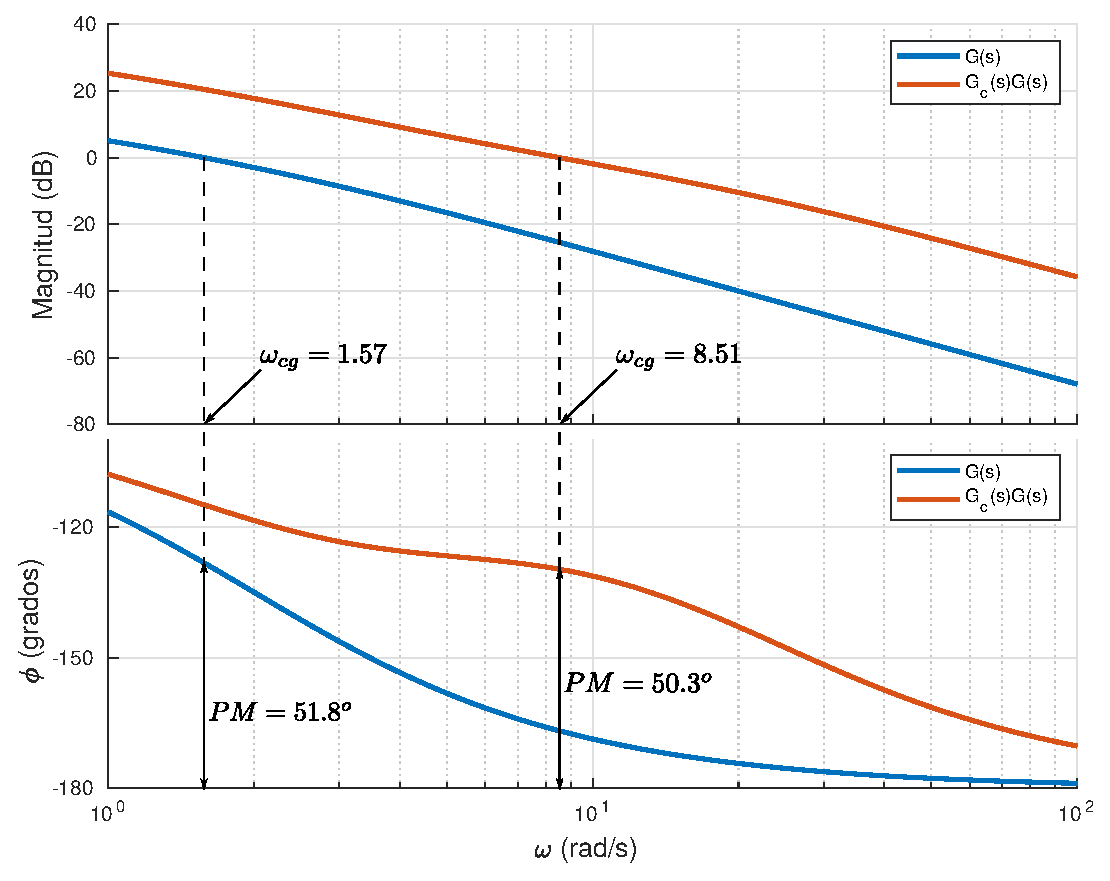
\includegraphics[width=9cm]{images/bodeLeadCompExampleComparison.eps}
		\end{figure}
	\end{column}
\end{columns}
\end{frame}

\begin{frame}[<+->]\frametitle{Compensador en Adelanto: Ejemplo - Respuesta Paso Sistema Compensado}
\begin{columns}
	\begin{column}{0.3\textwidth}
		El sistema compensado en lazo cerrado presenta una respuesta más rápida.
	\end{column}
	\begin{column}{0.7\textwidth}
		\begin{figure}
			\centering
			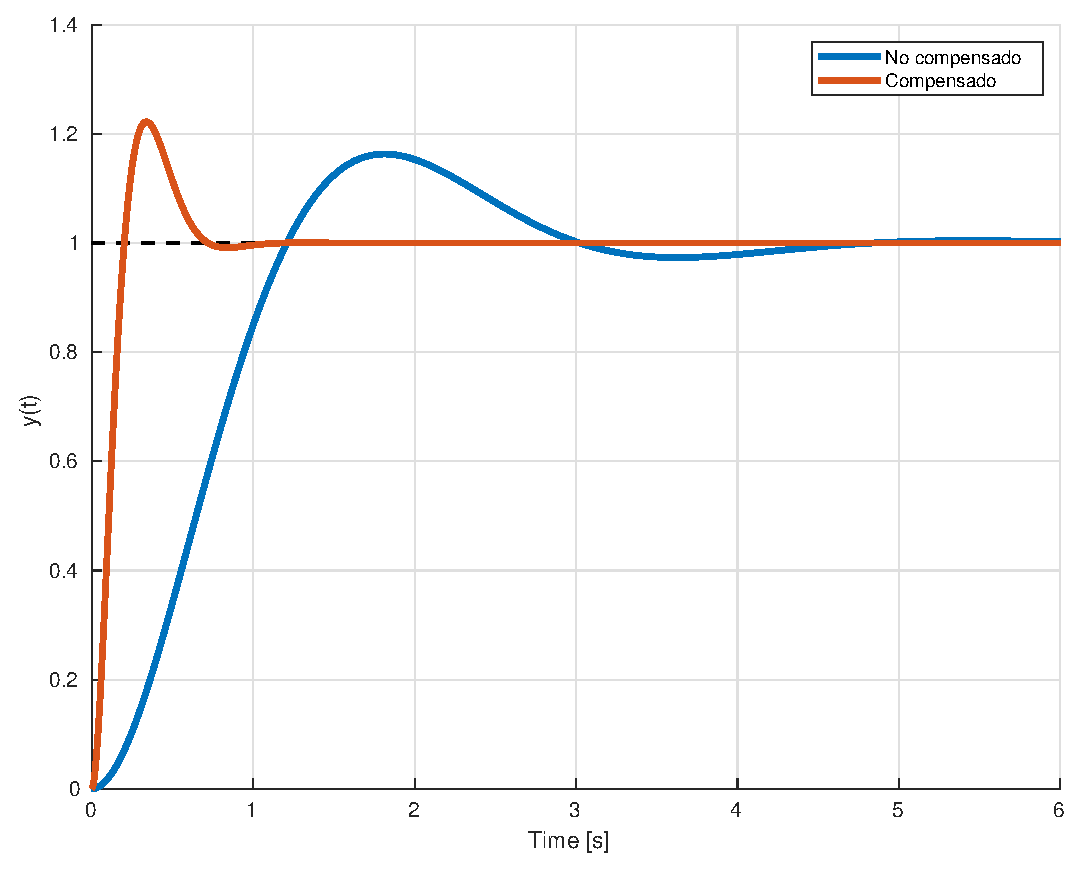
\includegraphics[width=9cm]{images/bodeLeadCompExampleStep.eps}
		\end{figure}
	\end{column}
\end{columns}
\end{frame}

\begin{frame}[<+->]\frametitle{Compensador en Adelanto: Ejemplo - Respuesta Rampa Sistema Compensado}
\vspace*{-2mm}
\begin{columns}
	\begin{column}{0.3\textwidth}
		El sistema compensado en lazo cerrado presenta un mejor seguimiento de la referencia rampa.
	\end{column}
	\begin{column}{0.7\textwidth}
		\begin{figure}
			\centering
			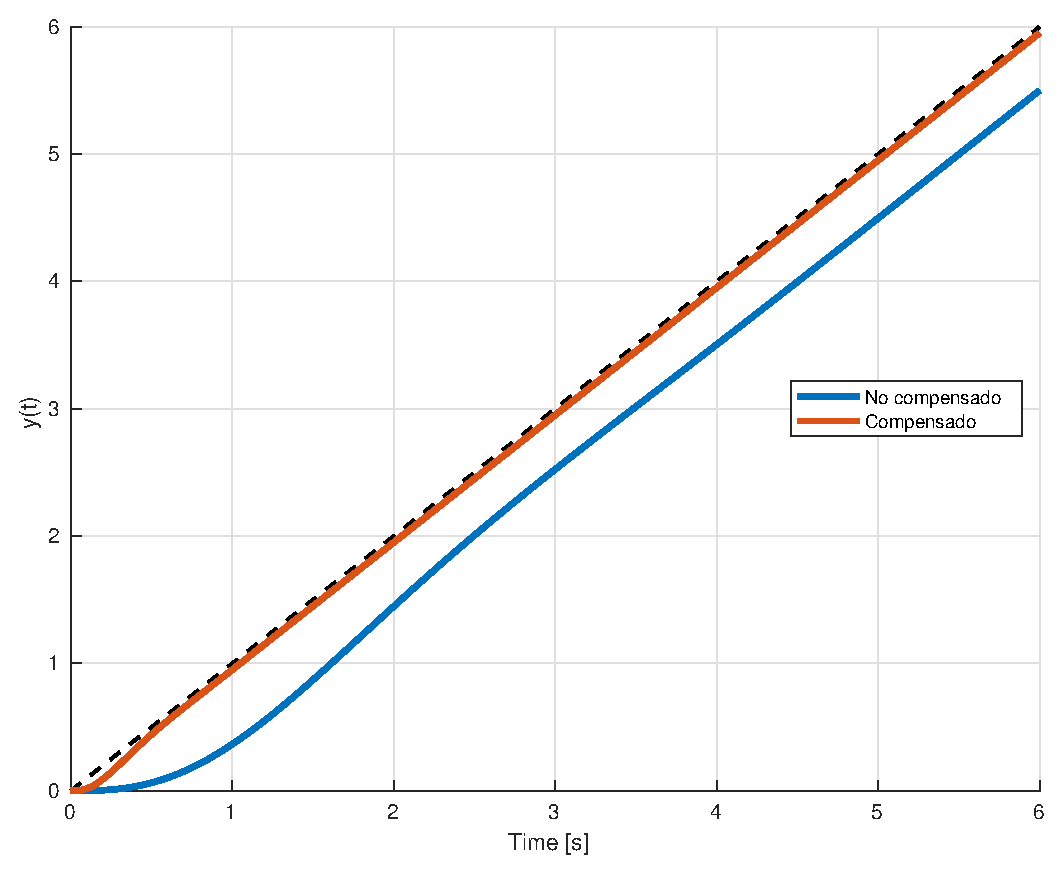
\includegraphics[width=9cm]{images/bodeLeadCompExampleRamp.eps}
		\end{figure}
	\end{column}
\end{columns}
\end{frame}

\begin{frame}[c]\frametitle{Taller}
\begin{enumerate}
	\item Considere el sistema mostrado en la figura. Dibuje el diagrama de Bode del sistema de lazo abierto a partir de los factores básicos de la función de transferencia. Compare el resultado con el gráfico obtenido usando la función \texttt{bode} de Matlab. Determine los márgenes de fase y ganancia del sistema.
	\begin{figure}
		\centering
		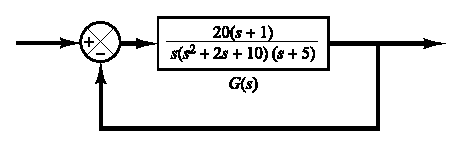
\includegraphics[width=6cm]{images/exercise1.eps}
	\end{figure}
	\seti 
\end{enumerate}
\end{frame}

\begin{frame}[c]\frametitle{Taller}
\begin{enumerate}
	\conti
	\item Considere un sistema de control con retroalimentación unitaria con la siguiente función de transferencia de lazo abierto:
	\begin{equation*}
		G(s) = \frac{K}{s(s^2+s+4)}
	\end{equation*}
	Determine el valor de la ganancia $K$ tal que el margen de fase sea \ang{50}. Cuál es el margen de ganancia para esta ganancia $K$?
	\seti 
\end{enumerate}
\end{frame}

\begin{frame}[c]\frametitle{Taller}
\begin{enumerate}
	\conti
	\item Considere el sistema mostrado en la figura. Dibuje el diagrama de Bode de la función de transferencia de lazo abierto y determine el valor de la ganancia K tal que el margen de fase sea \ang{50}. Cuál es el margen de ganancia del sistema con esta ganancia $K$?
	\begin{figure}
		\centering
		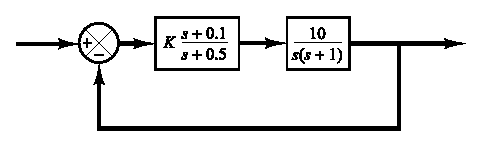
\includegraphics[width=8cm]{images/exercise3.eps}
	\end{figure}
	\seti 
\end{enumerate}
\end{frame}

\begin{frame}[c]\frametitle{Taller}
\begin{enumerate}
	\conti
	\item Considere el sistema de la figura. Se desea diseñar un compensador de adelanto $G_c(s)$ tal que el margen de fase sea $\ang{45}$, el márgen de fase no sea menor de 8 dB, y la constante de error de velocidad estática $K_v = 40$. Grafique las respuestas ante paso y rampa unitarias del sistema compensado.
	\begin{figure}
		\centering
		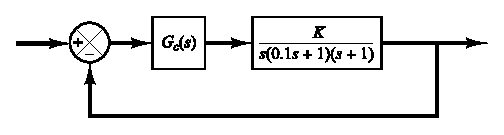
\includegraphics[width=8cm]{images/exercise4.eps}
	\end{figure}
	\seti 
\end{enumerate}
\end{frame}

\end{document}